\documentclass[a4paper,12pt]{report}
\usepackage[T1]{fontenc} 
\usepackage[french]{babel}

\usepackage[a4paper,top=2cm,bottom=2cm,left=3cm,right=3cm,marginparwidth=1.75cm]{geometry}

% Useful packages
\usepackage{amsmath, amsfonts, amssymb}
\usepackage{graphicx}
\usepackage{color}
\usepackage[colorlinks=true, allcolors=blue]{hyperref}
\usepackage{tikz}
\usepackage{pgfplots}
\usepackage{tikz}
\usetikzlibrary{3d,calc}
\pgfplotsset{compat=1.18}
\usepackage[utf8]{inputenc}
\usepackage{subcaption}
\setlength{\parskip}{1em}
\usepackage{cleveref}
\usepackage{enumitem}
\usepackage{animate}

\title{Rapport d'activités}
\author{Viet Anh QUACH}

\begin{document}
\maketitle
\tableofcontents

\setcounter{secnumdepth}{4}

\chapter{Étude bibliographique}
\section{Introduction de la thèse}
À cause du changement climatique, les risques naturels concernant l'écoulement gravitaire sur les zones montagneuses sont déclenchés de plus en plus fréquent à notre époque. 
Récemmement, Le village de Blatten, dans les Alpes suisses est rayé de la carte sous l'effet de L’éboulement du glacier le 29 mai 2025. 
Malhereusement, la caractéristique mécanique de ces phénomenes, reste mal comprise. 
Donc, mon projet de thèse, " Homogénéisation numérique à double échelle pour la modélisation demouvements gravitaires liés aux changements climatiques", se porte sur le développement d'une modélisation mécanique numérique pour l’écoulement de matériaux complexes. 
La méthodologie numérique pour réaliser ce simulation est basé sur La modélisation en intégrer 2 échelle simultané, qui consiste 2 processus hiérarchiques de each other. 
Pour cette homogénéisation, LA Méthode lagrangienne de Points Matériels (MPM) est choisisé à gestionner  La macroscopic, handle la mobilité du l'écoulement. 
meanwhile la microscopic, assuré par Méthode des éléments discrètes (DEM) jou la role de Loi Constitutive Homogénéisée Numériquement (LCHN). Le détail est illustré dans les sections suivante.

\section{MPM}
La Méthode de Point Matériel est une méthod numérical combiné Lagrangian particule et Eulerian maillage, used primarily dans dynamique de fluid. Parce que il est une Meshless Method(MME) or Meshfree Method, il provide solution of probmème in continuum mechanics while withstanding bien large déformation. 
Dans logiciels utilisant dans ce thèse, on utilise la méthode Updated Lagrangian MPM, which means la background maillage, composed by noeuds is fixed et the milieu granulaire deplacé parmi it. 
En effet, la noeud du maillage est déplacé pendant chaque étape calculation, though à leur terminaison, it came back to it premier position. Hence on peut dire la maillage est Eulerian, as mesh distortion never happens through out the simulation.
Le milieu granulaire est discretise aux matériels points, et chaque point matériel carries une certain volume de l'objet et tous les preoperties physique e.g mass, position, vélocité and variables nécessaire pour la constitutive relation.
Therefore les points est dans la Lagrangian framework, providing the state of the body at any time step \cite{danies2018application}.
L'algorithme de base sur la ULMPM consiste de 4 steps principale:
\begin{enumerate}
\item À l'instant $t$, les informations de particules sont transférées vers les nœuds correspondants dans leur zone d'affectation sur le maillage.
\item L'équation de la quantité de mouvement est résolue aux nœuds et les propriétés des nœuds sont mises à jour.
\item Les informations sont transférées des nœuds mis à jour vers les particules, mettant à jour leurs propriétés (position, vélocité, contrainte, déformation, etc.).
\item Le maillage est réinitialisé à la position initiale, et on continue le cycle à l'instant suivant $t + \delta t$.
\end{enumerate}

\section{DEM}
Originé de Molécular Dynamic, Discrète ÉLEMENTS MÉTHODE a pour objectif d’étudier les problèmes mis en jeu dans les matériaux granulaires et les géomatériaux. En revanche de méthode continuum as MPM ou FEM, Cette méthode approche le milieu granulaire comme les particules discrète.
L’approche par DEM considère le milieu est assembmage de grains indépendamment les uns des autres et consiste à intégrer le mouvement des grains décrit par l’équation de la deuxième loi de Newton. pendant chaque pas de temps discrete, équation de équilibration sur grain $i$ denoted as : $F_i = m_i \dfrac{d^2x_i}{dt^2}, i = 1,\dots,N$.  
C’est pourquoi on l’appelle aussi la famille des méthodes Newtoniennes.
GRace à DEM, tous les effect de forces intergranulaire est capable de captured et ingetated selon la demande de bai toan. $F_i$ co the bao gom:
\begin{itemize}[label=$\bullet$]
    \item Composant $F_{ij}$ est la force exercée par les grains $j$ en contact avec $i$, qui consiste en :
    \begin{itemize}[label=$\cdot$]
        \item la force normale ($f_n$): Composante élastique ($f_{n,\mathrm{elas}}$), Composante d’amortissement ($f_{n,\mathrm{v}}$), Composante de liaison ($f_{n,\mathrm{bond}}$), Composante de cohésion de surface($f_{\mathrm{coh}}$)
        \item la force tangentielle ($f_t$): Composante de frottement ($f_{t,\mathrm{fric}}$),Composante de liaison ($f_{t,\mathrm{bond}}$) 
        \item la Moment ($M$)
    \end{itemize}
    \item Composant force externe $F_{ext}$ peut inclure :
    \begin{itemize}
        \item la force de gravité
        \item la force d'Archimède dans un milieu de l'eau
        \item \dots etc
    \end{itemize}
\end{itemize} 
Dans l'étude actuellement, la shape de grain est sphere 3D mais One peut changer la taille, shape, rigidité, ou bien quelle indice qui s'adapté au matériau d'étude le plus précis. 
C'est possible de diviser simplement l'algorithme de DEM en aussi 4 steps principale:
\begin{enumerate}
\item À l'instant $t$, avec la liste de position de graines, vérifions nous les contacts entre elles
\item Calcul du torseur sur chaque grain 
\item  Dung phuong trinh II Newton pour obtenir leurs accelation
\item Calcul la position de particules à l'instant suivant $t + \delta t$ et on continue le cycle
\end{enumerate}


\section{Couplage MPMxDEM}
\begin{figure}[h]
\centering
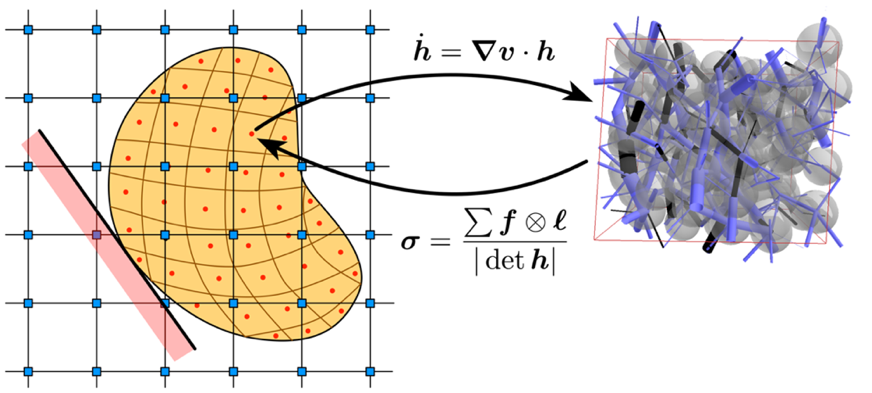
\includegraphics[width=0.5\textwidth]{CouplageMPMxDEM.png}
\caption{Principe d’une approche à deux échelles hiérarchiques.\cite{projetderecherche}}
\label{fig:MPMxDEM}
\end{figure}
Effectivement, La couplage entre 2 méthodes différents has been used prevelantly est efficacely, sans peut pas ignorer comme \emph{text} x DEM \cite{nguyen2013modelisation}. 
Mais pour résourdre ce probleme du écoulement granulaire, les 2 adopté méthodes bright shinely et apporte des avantages significatifs.
For instance, comme indiqué dans \autoref{fig:MPMxDEM}, la MPM (La partie à gauche) prends en charge de la computation du gradient de déformation $\nabla v$, envoyant au points mattériel (rouge) qui represent maintenant par une volume element represent (VER) DEM à calculer la tensor du contrainte $\sigma_p$ selon la formulation de LOVE,WEBER.
Grace à l'acces du DEM, la résolution important du petit échelle est accesiblé et manipulé liberté afin de s'adapter au complexité du matériaux modelisé. 
Ca permettre d'une mieux solution comparant avec une loi de constitutive calculus thong thuong.
En meme temps, MPM reduit la complexité du prix chère du calcul en le considérant comme un object total mais sans facer à la subis de grand déformation qui distorte la maillage comme FEM.
When combining, les deux méthode preserve their own advantages whereas cover each other weekness.
Au laboratoire 3SR, deux programmes de calcul en C++ pour la MPM et la DEM s'appellent respectivement ``MPMbox'' et ``3D\_sandstone'' et leur intégration est bien implémentée~\cite{richefeu2025mpmxdem}.
La modélisation est aussi réalisée et prouvée précise, mais il reste encore des verrous à surmonter:
\begin{itemize}
    \item Équivalence des inerties aux deux échelles : Indeed, MPM qui a été developpé pour handle des problemes contact rapide des objets \cite{nguyen2023material.}, porte bien l'effet dynamique. En revanche, DEM censure les réponses mécaniques dynamiques en attendant une stabilisation statique systématique \cite{nguyen2014fem}. Leur couplage fait emerge des Diverses nouvelles interrogations théoriques sur l'équivalence des inerties aux deux échelles together en meme temps, when it comes to computational calcul for a granular flow which is highly dynamic.
    \item Conditions aux limites et initiales~: spécifiquement, dans la simulation DEM, la partie de condition aux limites périodiques n'est pas réalisée de manière pleinement satisfaisante, ce qui pose des pics abnormaux de contrainte.
\end{itemize}

% \section{Compétences soutenues}
% \begin{itemize}
%       \item C++
%       \item Gnuplot
%       \item LaTeX
%       \item % Inkscape
% % Writing thesis
% % 120 formations sur ADUM
% % Linux
% % Clavier français :D
% \end{itemize}


\chapter{L'étude pratique}
\section{Simulation MPM}
\subsection{Étude sur le cas statique - Déformation d'une poutre console}
En raison de vérifier la juste de la programme MPM, une poutre encastre console qui se deforme sous l'effet de self mass (gravité) est chosise à modeled. 
On vérifie d'abord avec la loi de constitutive Hooke, d'autre dire loi elastic by comparison avec la équation calculus de resistance de materiaux.
\begin{figure}[h]
\centering
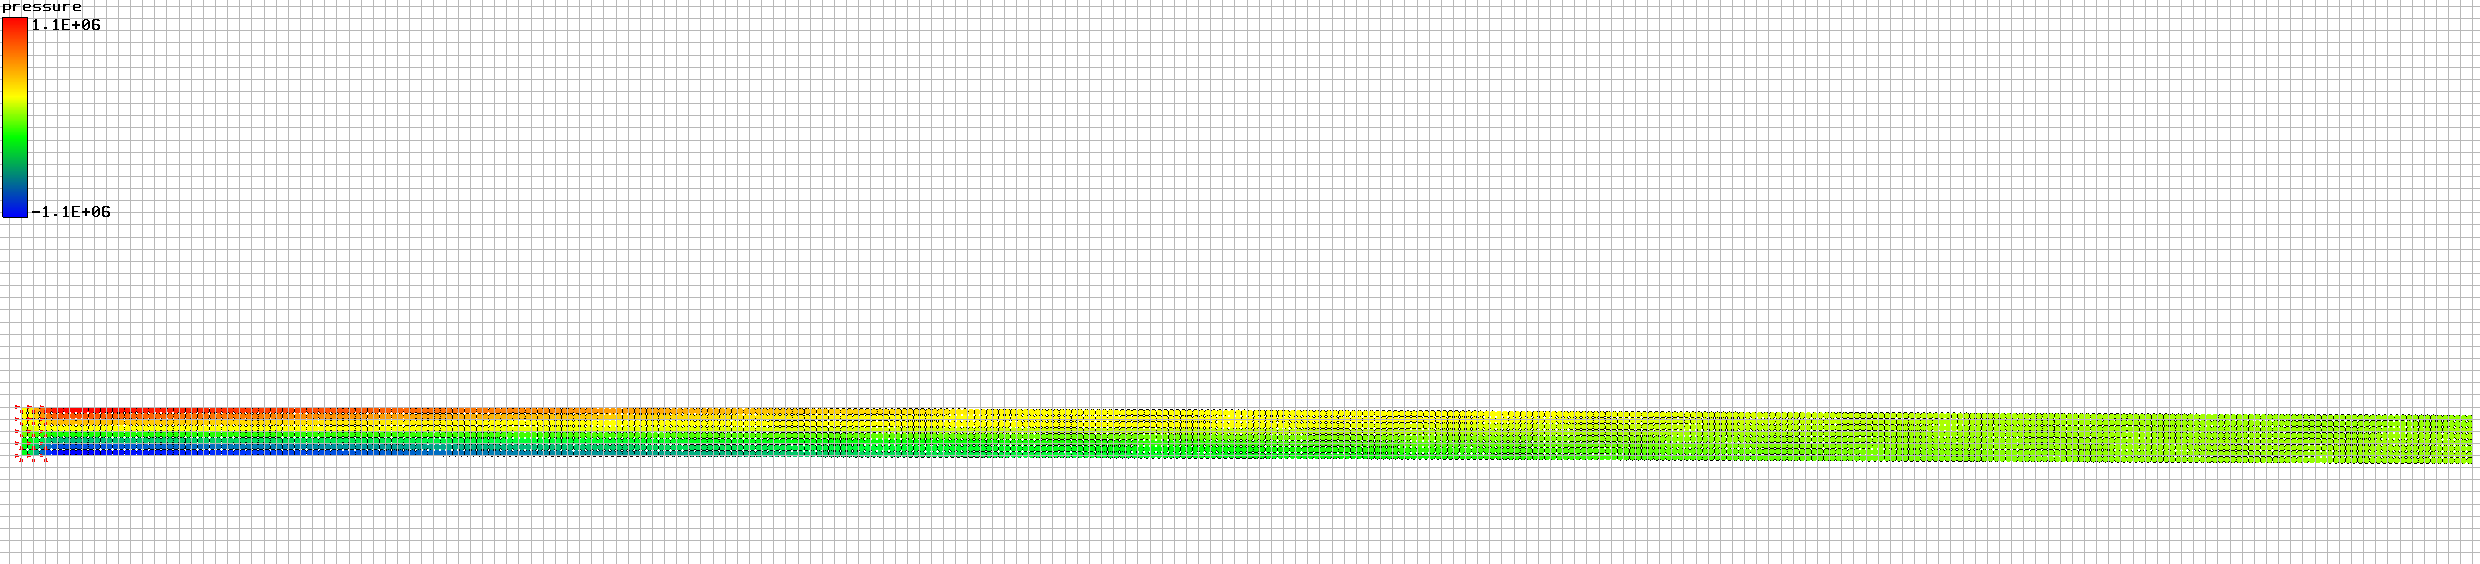
\includegraphics[height=0.13\textheight]{Model_Poutre.png}
\caption{Principe d’une approche à deux échelles hiérarchiques.\cite{projetderecherche}}
\label{fig:ModelPoutre}
\end{figure}
\begin{figure}[h]
    \centering
    \small
    % GNUPLOT: LaTeX picture with Postscript
\begingroup
  \makeatletter
  \providecommand\color[2][]{%
    \GenericError{(gnuplot) \space\space\space\@spaces}{%
      Package color not loaded in conjunction with
      terminal option `colourtext'%
    }{See the gnuplot documentation for explanation.%
    }{Either use 'blacktext' in gnuplot or load the package
      color.sty in LaTeX.}%
    \renewcommand\color[2][]{}%
  }%
  \providecommand\includegraphics[2][]{%
    \GenericError{(gnuplot) \space\space\space\@spaces}{%
      Package graphicx or graphics not loaded%
    }{See the gnuplot documentation for explanation.%
    }{The gnuplot epslatex terminal needs graphicx.sty or graphics.sty.}%
    \renewcommand\includegraphics[2][]{}%
  }%
  \providecommand\rotatebox[2]{#2}%
  \@ifundefined{ifGPcolor}{%
    \newif\ifGPcolor
    \GPcolortrue
  }{}%
  \@ifundefined{ifGPblacktext}{%
    \newif\ifGPblacktext
    \GPblacktextfalse
  }{}%
  % define a \g@addto@macro without @ in the name:
  \let\gplgaddtomacro\g@addto@macro
  % define empty templates for all commands taking text:
  \gdef\gplbacktext{}%
  \gdef\gplfronttext{}%
  \makeatother
  \ifGPblacktext
    % no textcolor at all
    \def\colorrgb#1{}%
    \def\colorgray#1{}%
  \else
    % gray or color?
    \ifGPcolor
      \def\colorrgb#1{\color[rgb]{#1}}%
      \def\colorgray#1{\color[gray]{#1}}%
      \expandafter\def\csname LTw\endcsname{\color{white}}%
      \expandafter\def\csname LTb\endcsname{\color{black}}%
      \expandafter\def\csname LTa\endcsname{\color{black}}%
      \expandafter\def\csname LT0\endcsname{\color[rgb]{1,0,0}}%
      \expandafter\def\csname LT1\endcsname{\color[rgb]{0,1,0}}%
      \expandafter\def\csname LT2\endcsname{\color[rgb]{0,0,1}}%
      \expandafter\def\csname LT3\endcsname{\color[rgb]{1,0,1}}%
      \expandafter\def\csname LT4\endcsname{\color[rgb]{0,1,1}}%
      \expandafter\def\csname LT5\endcsname{\color[rgb]{1,1,0}}%
      \expandafter\def\csname LT6\endcsname{\color[rgb]{0,0,0}}%
      \expandafter\def\csname LT7\endcsname{\color[rgb]{1,0.3,0}}%
      \expandafter\def\csname LT8\endcsname{\color[rgb]{0.5,0.5,0.5}}%
    \else
      % gray
      \def\colorrgb#1{\color{black}}%
      \def\colorgray#1{\color[gray]{#1}}%
      \expandafter\def\csname LTw\endcsname{\color{white}}%
      \expandafter\def\csname LTb\endcsname{\color{black}}%
      \expandafter\def\csname LTa\endcsname{\color{black}}%
      \expandafter\def\csname LT0\endcsname{\color{black}}%
      \expandafter\def\csname LT1\endcsname{\color{black}}%
      \expandafter\def\csname LT2\endcsname{\color{black}}%
      \expandafter\def\csname LT3\endcsname{\color{black}}%
      \expandafter\def\csname LT4\endcsname{\color{black}}%
      \expandafter\def\csname LT5\endcsname{\color{black}}%
      \expandafter\def\csname LT6\endcsname{\color{black}}%
      \expandafter\def\csname LT7\endcsname{\color{black}}%
      \expandafter\def\csname LT8\endcsname{\color{black}}%
    \fi
  \fi
    \setlength{\unitlength}{0.0500bp}%
    \ifx\gptboxheight\undefined%
      \newlength{\gptboxheight}%
      \newlength{\gptboxwidth}%
      \newsavebox{\gptboxtext}%
    \fi%
    \setlength{\fboxrule}{0.5pt}%
    \setlength{\fboxsep}{1pt}%
    \definecolor{tbcol}{rgb}{1,1,1}%
\begin{picture}(7200.00,5040.00)%
    \gplgaddtomacro\gplbacktext{%
      \csname LTb\endcsname%%
      \put(682,704){\makebox(0,0)[r]{\strut{}$-5$}}%
      \csname LTb\endcsname%%
      \put(682,1390){\makebox(0,0)[r]{\strut{}$-4$}}%
      \csname LTb\endcsname%%
      \put(682,2076){\makebox(0,0)[r]{\strut{}$-3$}}%
      \csname LTb\endcsname%%
      \put(682,2762){\makebox(0,0)[r]{\strut{}$-2$}}%
      \csname LTb\endcsname%%
      \put(682,3447){\makebox(0,0)[r]{\strut{}$-1$}}%
      \csname LTb\endcsname%%
      \put(682,4133){\makebox(0,0)[r]{\strut{}$0$}}%
      \csname LTb\endcsname%%
      \put(682,4819){\makebox(0,0)[r]{\strut{}$1$}}%
      \csname LTb\endcsname%%
      \put(814,484){\makebox(0,0){\strut{}$0$}}%
      \csname LTb\endcsname%%
      \put(2012,484){\makebox(0,0){\strut{}$0.2$}}%
      \csname LTb\endcsname%%
      \put(3210,484){\makebox(0,0){\strut{}$0.4$}}%
      \csname LTb\endcsname%%
      \put(4407,484){\makebox(0,0){\strut{}$0.6$}}%
      \csname LTb\endcsname%%
      \put(5605,484){\makebox(0,0){\strut{}$0.8$}}%
      \csname LTb\endcsname%%
      \put(6803,484){\makebox(0,0){\strut{}$1$}}%
    }%
    \gplgaddtomacro\gplfronttext{%
      \csname LTb\endcsname%%
      \put(209,2761){\rotatebox{-270}{\makebox(0,0){\strut{}$f_y$ (mm)}}}%
      \put(3808,154){\makebox(0,0){\strut{}$x$ (m)}}%
      \csname LTb\endcsname%%
      \put(6009,4493){\makebox(0,0)[r]{\strut{}$\text{f}_{\text{calcul}}$}}%
      \csname LTb\endcsname%%
      \put(6009,4373){\makebox(0,0)[r]{\strut{}$\text{f}_{\text{théorique}}$}}%
      \csname LTb\endcsname%%
      \put(3808,33733){\makebox(0,0){\strut{}}}%
    }%
    \gplbacktext
    \put(0,0){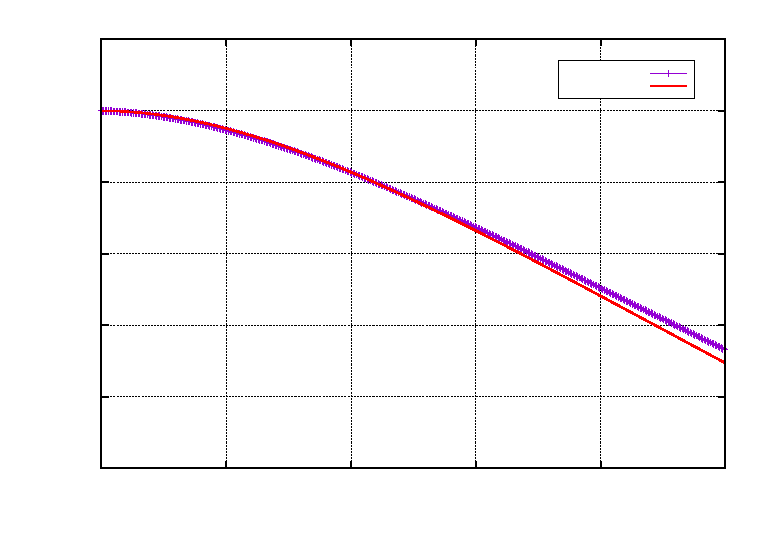
\includegraphics[width={360.00bp},height={252.00bp}]{./Deplacement_Poutre}}%
    \gplfronttext
  \end{picture}%
\endgroup

    \caption{Déplacement de la poutre selon l’axe Y}
    \label{fig:deplacementPoutre}
\end{figure}

La flèche $f$ de la poutre est donnée par :

\begin{equation}
    f = \dfrac{-qx^2}{24EI} \times (x^2 - 4Lx + 6L^2)
    \label{eq:fleche}
\end{equation}

où $q$ représente la charge uniformément répartie sur la longueur de la poutre, $x$ est la position considérée, $I$ est le moment d'inertie, et $E$ est le module de Young.

On constate que la flèche calculée analytiquement selon l'équation théorique \eqref{eq:fleche} est en bon accord avec la déformation obtenue numériquement, comme le montre la ~\autoref{fig:deplacementPoutre}.
C'est worth to noted that the longeur d'encastre and the discretasion du maillage dans ce modélisation MPM doit s'adapte au scale du objet.


²\subsection{Étude sur le cas dynamique}



\section{Simulation DEM: Compression triaxiale}

    \begin{figure}[h]
        \centering
        \animategraphics[loop,autoplay,width=5cm]{10}{Triaxial_}{1}{8}
        \caption{Déformation de la boite}
        \label{fig:boiteDeformation}
    \end{figure}
On conduit la triaxiale test dans la section DEM, qui consiste de 2 étape: 
\begin{itemize}
\item préparation du échantillon: Prenons un échantillons - un box qui hold multiple non cohésion sphere particle inside, effectuons un processus de compression isotrope, avec différentes valeurs du coefficient de frottement $\mu$. 
Dieu nay dan den la varies du dispersion du particule, creer des different echantillons de denses a lache according to evolution du $\mu$.
\item prenant la sample obtenue de la precessus précédent, ilpmique une pression de confinement constante et une vitesse de déformation axiale imposée constante sur l'axe yy (la déformation du boite est dans la \autoref{fig:boiteDeformation}). 
Premierement les caracteistique mecanique khac nhau according to luc chuan bi mau est observée.
Deuxiememmn , as to be integraté dans la simulation DEMxMPM, l'etude sur la inertie est la main focus. échantillons est compressé dans une grande vitess, d'autre dire avec un grande nombre d'inertie.
\end{itemize}
\subsection{Le processus et les paramètres}
\begin{frame}{Étude sur le critère de rupture de Coulomb}
\begin{table}
\centering
\begin{tabular}{|c|c|c|c|}
\hline
\textbf{Symboles} & \textbf{Paramètres} & \textbf{Valeurs} & \textbf{Unité} \\ 
\hline
Nombre de particules & N & $15^3$ & $-$ \\  
\hline
Le rayon des particules & R & 0.003 $\div$ 0.005 & m \\  
\hline
Masse volumique & $\rho$  & 2500 & $kg/m^3$ \\
\hline
Contrainte isotrope & $\sigma_{xx} = \sigma_{zz}$ & 100, 200, 300 & kPa \\ 
\hline
Raideur normale et tangentielle & $k_n$ \& $k_t$ & $10^6, 2 \times 10^6, 3 \times 10^6$ & N/m \\ 
\hline
Niveau de raideur & $\kappa$ & 1000 & $-$ \\  
\hline
Coefficient de frottement & $\mu$ & 0.0 \& 0.4 & $-$ \\ 
\hline
Coefficient d'amortissement & $\alpha$  & 0.7 & $-$\\
\hline
\end{tabular}
\caption{Valeurs des paramètres utilisés dans la compression isotrope.}
\end{table}

\[
\text{Générer l'échantillon dense} \rightarrow \text{Compression isotrope} \rightarrow \text{Compression triaxiale}
\]
\end{frame}

\begin{frame}{Étude sur le critère de rupture de Coulomb (Roche)}
\begin{table}
\centering
\begin{tabular}{|c|c|c|c|}
\hline
\textbf{Symboles} & \textbf{Paramètres} & \textbf{Valeurs} & \textbf{Unité} \\ 
\hline
Nombre de particules & N & $15^3$ & $-$ \\  
\hline
Le rayon des particules & R & 0.003 $\div$ 0.005 & m \\  
\hline
Masse volumique & $\rho$  & 2500 & $kg/m^3$ \\
\hline
Contrainte isotrope & $\sigma_{xx} = \sigma_{zz}$ & 100, 200, 300 & kPa \\ 
\hline
Raideur normale et tangentielle & $k_n$ \& $k_t$ & $10^6, 2 \times 10^6, 3 \times 10^6$ & N/m \\ 
\hline
Niveau de raideur & $\kappa$ & 1000 & $-$ \\ 
\hline
Coefficient de frottement & $\mu$ & 0.5 & $-$ \\ 
\hline
Déformation axiale & $\varepsilon_{\text{yy}}$ &  10 & $\%$ \\ 
\hline
Nombre d’inertie & I & $10^{-3}$ & $-$ \\ 
\hline
Vitess imposéee & v & $10^{-3} \& 10^{-1}$ & m/s \\ 
\hline
Pas de temps & $d_t$  & $10^{-6} \& 10^{-8}$ & $-$\\
\hline
Taux de amortissement & $\frac{\eta}{\eta_{\max}}$  & 0.95 & $-$\\
\hline
\end{tabular}
\caption{Valeurs des paramètres utilisés dans la compression triaxiale}
\end{table}
\end{frame}
\subsection{Les caractéristiques mécaniques générales du sol}
\subsubsection{La granulométrie et la fraction solide}
La fraction solide caractère la dispersion des particules solide $V_s$ dans une volumne $V$.
\begin{equation}
\Phi = \dfrac{V_s}{V} = \dfrac{\sum\limits_{i = 1}^n \frac{4}{3}\pi R_i^3}{\det(h)}
\end{equation}
                                \begin{figure}
                                   \centering \small % GNUPLOT: LaTeX picture with Postscript
\begingroup
  \makeatletter
  \providecommand\color[2][]{%
    \GenericError{(gnuplot) \space\space\space\@spaces}{%
      Package color not loaded in conjunction with
      terminal option `colourtext'%
    }{See the gnuplot documentation for explanation.%
    }{Either use 'blacktext' in gnuplot or load the package
      color.sty in LaTeX.}%
    \renewcommand\color[2][]{}%
  }%
  \providecommand\includegraphics[2][]{%
    \GenericError{(gnuplot) \space\space\space\@spaces}{%
      Package graphicx or graphics not loaded%
    }{See the gnuplot documentation for explanation.%
    }{The gnuplot epslatex terminal needs graphicx.sty or graphics.sty.}%
    \renewcommand\includegraphics[2][]{}%
  }%
  \providecommand\rotatebox[2]{#2}%
  \@ifundefined{ifGPcolor}{%
    \newif\ifGPcolor
    \GPcolortrue
  }{}%
  \@ifundefined{ifGPblacktext}{%
    \newif\ifGPblacktext
    \GPblacktextfalse
  }{}%
  % define a \g@addto@macro without @ in the name:
  \let\gplgaddtomacro\g@addto@macro
  % define empty templates for all commands taking text:
  \gdef\gplbacktext{}%
  \gdef\gplfronttext{}%
  \makeatother
  \ifGPblacktext
    % no textcolor at all
    \def\colorrgb#1{}%
    \def\colorgray#1{}%
  \else
    % gray or color?
    \ifGPcolor
      \def\colorrgb#1{\color[rgb]{#1}}%
      \def\colorgray#1{\color[gray]{#1}}%
      \expandafter\def\csname LTw\endcsname{\color{white}}%
      \expandafter\def\csname LTb\endcsname{\color{black}}%
      \expandafter\def\csname LTa\endcsname{\color{black}}%
      \expandafter\def\csname LT0\endcsname{\color[rgb]{1,0,0}}%
      \expandafter\def\csname LT1\endcsname{\color[rgb]{0,1,0}}%
      \expandafter\def\csname LT2\endcsname{\color[rgb]{0,0,1}}%
      \expandafter\def\csname LT3\endcsname{\color[rgb]{1,0,1}}%
      \expandafter\def\csname LT4\endcsname{\color[rgb]{0,1,1}}%
      \expandafter\def\csname LT5\endcsname{\color[rgb]{1,1,0}}%
      \expandafter\def\csname LT6\endcsname{\color[rgb]{0,0,0}}%
      \expandafter\def\csname LT7\endcsname{\color[rgb]{1,0.3,0}}%
      \expandafter\def\csname LT8\endcsname{\color[rgb]{0.5,0.5,0.5}}%
    \else
      % gray
      \def\colorrgb#1{\color{black}}%
      \def\colorgray#1{\color[gray]{#1}}%
      \expandafter\def\csname LTw\endcsname{\color{white}}%
      \expandafter\def\csname LTb\endcsname{\color{black}}%
      \expandafter\def\csname LTa\endcsname{\color{black}}%
      \expandafter\def\csname LT0\endcsname{\color{black}}%
      \expandafter\def\csname LT1\endcsname{\color{black}}%
      \expandafter\def\csname LT2\endcsname{\color{black}}%
      \expandafter\def\csname LT3\endcsname{\color{black}}%
      \expandafter\def\csname LT4\endcsname{\color{black}}%
      \expandafter\def\csname LT5\endcsname{\color{black}}%
      \expandafter\def\csname LT6\endcsname{\color{black}}%
      \expandafter\def\csname LT7\endcsname{\color{black}}%
      \expandafter\def\csname LT8\endcsname{\color{black}}%
    \fi
  \fi
    \setlength{\unitlength}{0.0500bp}%
    \ifx\gptboxheight\undefined%
      \newlength{\gptboxheight}%
      \newlength{\gptboxwidth}%
      \newsavebox{\gptboxtext}%
    \fi%
    \setlength{\fboxrule}{0.5pt}%
    \setlength{\fboxsep}{1pt}%
    \definecolor{tbcol}{rgb}{1,1,1}%
\begin{picture}(7200.00,5040.00)%
    \gplgaddtomacro\gplbacktext{%
      \csname LTb\endcsname%%
      \put(946,704){\makebox(0,0)[r]{\strut{}$0.56$}}%
      \csname LTb\endcsname%%
      \put(946,1218){\makebox(0,0)[r]{\strut{}$0.57$}}%
      \csname LTb\endcsname%%
      \put(946,1733){\makebox(0,0)[r]{\strut{}$0.58$}}%
      \csname LTb\endcsname%%
      \put(946,2247){\makebox(0,0)[r]{\strut{}$0.59$}}%
      \csname LTb\endcsname%%
      \put(946,2762){\makebox(0,0)[r]{\strut{}$0.6$}}%
      \csname LTb\endcsname%%
      \put(946,3276){\makebox(0,0)[r]{\strut{}$0.61$}}%
      \csname LTb\endcsname%%
      \put(946,3790){\makebox(0,0)[r]{\strut{}$0.62$}}%
      \csname LTb\endcsname%%
      \put(946,4305){\makebox(0,0)[r]{\strut{}$0.63$}}%
      \csname LTb\endcsname%%
      \put(946,4819){\makebox(0,0)[r]{\strut{}$0.64$}}%
      \csname LTb\endcsname%%
      \put(1598,484){\makebox(0,0){\strut{}$0.1$}}%
      \csname LTb\endcsname%%
      \put(2177,484){\makebox(0,0){\strut{}$0.2$}}%
      \csname LTb\endcsname%%
      \put(2755,484){\makebox(0,0){\strut{}$0.3$}}%
      \csname LTb\endcsname%%
      \put(3333,484){\makebox(0,0){\strut{}$0.4$}}%
      \csname LTb\endcsname%%
      \put(3912,484){\makebox(0,0){\strut{}$0.5$}}%
      \csname LTb\endcsname%%
      \put(4490,484){\makebox(0,0){\strut{}$0.6$}}%
      \csname LTb\endcsname%%
      \put(5068,484){\makebox(0,0){\strut{}$0.7$}}%
      \csname LTb\endcsname%%
      \put(5646,484){\makebox(0,0){\strut{}$0.8$}}%
      \csname LTb\endcsname%%
      \put(6225,484){\makebox(0,0){\strut{}$0.9$}}%
      \csname LTb\endcsname%%
      \put(6803,484){\makebox(0,0){\strut{}$1$}}%
    }%
    \gplgaddtomacro\gplfronttext{%
      \csname LTb\endcsname%%
      \put(209,2761){\rotatebox{-270}{\makebox(0,0){\strut{}$\Phi$}}}%
      \put(3940,154){\makebox(0,0){\strut{}$\mu$}}%
      \csname LTb\endcsname%%
      \put(3940,26625){\makebox(0,0){\strut{}}}%
    }%
    \gplbacktext
    \put(0,0){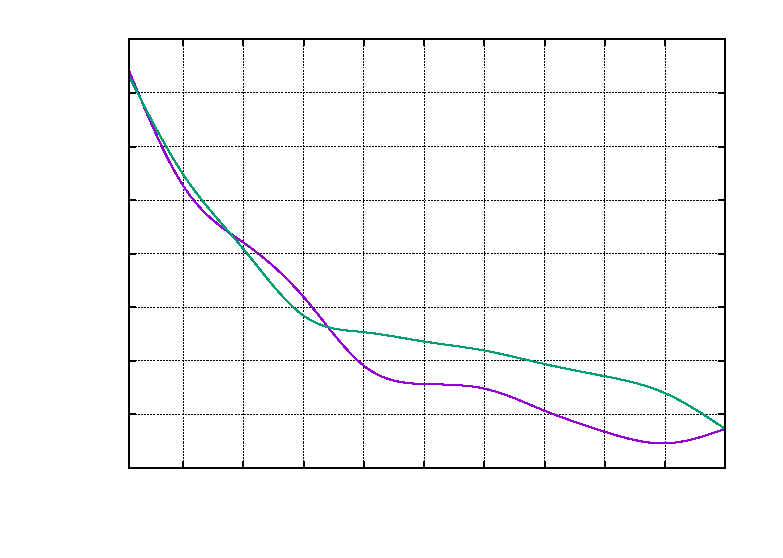
\includegraphics[width={360.00bp},height={252.00bp}]{./fractonSolide}}%
    \gplfronttext
  \end{picture}%
\endgroup

                                    \caption{La fraction solide}
                                    \label{fig:fractionSolideMax}
                                \end{figure}

La \autoref{fig:fractionSolideMax} montre que leur valeur maximale $\Phi_{\max}$ pour une dispersion désordonnée de sphères en contact dense est approximée à 0.64~\cite{combe2023demlecture}.
\subsubsection{Les caractéristiques des échantillons denses}
\subsubsection{Les caractéristiques des échantillons lâches}
\subsubsection{L'état critique}
\begin{figure}[htbp]
    \centering
    \begin{subfigure}[b]{0.49\textwidth}
        \centering \small
        \scalebox{0.5}{% GNUPLOT: LaTeX picture with Postscript
\begingroup
  \makeatletter
  \providecommand\color[2][]{%
    \GenericError{(gnuplot) \space\space\space\@spaces}{%
      Package color not loaded in conjunction with
      terminal option `colourtext'%
    }{See the gnuplot documentation for explanation.%
    }{Either use 'blacktext' in gnuplot or load the package
      color.sty in LaTeX.}%
    \renewcommand\color[2][]{}%
  }%
  \providecommand\includegraphics[2][]{%
    \GenericError{(gnuplot) \space\space\space\@spaces}{%
      Package graphicx or graphics not loaded%
    }{See the gnuplot documentation for explanation.%
    }{The gnuplot epslatex terminal needs graphicx.sty or graphics.sty.}%
    \renewcommand\includegraphics[2][]{}%
  }%
  \providecommand\rotatebox[2]{#2}%
  \@ifundefined{ifGPcolor}{%
    \newif\ifGPcolor
    \GPcolortrue
  }{}%
  \@ifundefined{ifGPblacktext}{%
    \newif\ifGPblacktext
    \GPblacktexttrue
  }{}%
  % define a \g@addto@macro without @ in the name:
  \let\gplgaddtomacro\g@addto@macro
  % define empty templates for all commands taking text:
  \gdef\gplbacktext{}%
  \gdef\gplfronttext{}%
  \makeatother
  \ifGPblacktext
    % no textcolor at all
    \def\colorrgb#1{}%
    \def\colorgray#1{}%
  \else
    % gray or color?
    \ifGPcolor
      \def\colorrgb#1{\color[rgb]{#1}}%
      \def\colorgray#1{\color[gray]{#1}}%
      \expandafter\def\csname LTw\endcsname{\color{white}}%
      \expandafter\def\csname LTb\endcsname{\color{black}}%
      \expandafter\def\csname LTa\endcsname{\color{black}}%
      \expandafter\def\csname LT0\endcsname{\color[rgb]{1,0,0}}%
      \expandafter\def\csname LT1\endcsname{\color[rgb]{0,1,0}}%
      \expandafter\def\csname LT2\endcsname{\color[rgb]{0,0,1}}%
      \expandafter\def\csname LT3\endcsname{\color[rgb]{1,0,1}}%
      \expandafter\def\csname LT4\endcsname{\color[rgb]{0,1,1}}%
      \expandafter\def\csname LT5\endcsname{\color[rgb]{1,1,0}}%
      \expandafter\def\csname LT6\endcsname{\color[rgb]{0,0,0}}%
      \expandafter\def\csname LT7\endcsname{\color[rgb]{1,0.3,0}}%
      \expandafter\def\csname LT8\endcsname{\color[rgb]{0.5,0.5,0.5}}%
    \else
      % gray
      \def\colorrgb#1{\color{black}}%
      \def\colorgray#1{\color[gray]{#1}}%
      \expandafter\def\csname LTw\endcsname{\color{white}}%
      \expandafter\def\csname LTb\endcsname{\color{black}}%
      \expandafter\def\csname LTa\endcsname{\color{black}}%
      \expandafter\def\csname LT0\endcsname{\color{black}}%
      \expandafter\def\csname LT1\endcsname{\color{black}}%
      \expandafter\def\csname LT2\endcsname{\color{black}}%
      \expandafter\def\csname LT3\endcsname{\color{black}}%
      \expandafter\def\csname LT4\endcsname{\color{black}}%
      \expandafter\def\csname LT5\endcsname{\color{black}}%
      \expandafter\def\csname LT6\endcsname{\color{black}}%
      \expandafter\def\csname LT7\endcsname{\color{black}}%
      \expandafter\def\csname LT8\endcsname{\color{black}}%
    \fi
  \fi
    \setlength{\unitlength}{0.0500bp}%
    \ifx\gptboxheight\undefined%
      \newlength{\gptboxheight}%
      \newlength{\gptboxwidth}%
      \newsavebox{\gptboxtext}%
    \fi%
    \setlength{\fboxrule}{0.5pt}%
    \setlength{\fboxsep}{1pt}%
    \definecolor{tbcol}{rgb}{1,1,1}%
\begin{picture}(7200.00,5040.00)%
    \gplgaddtomacro\gplbacktext{%
      \csname LTb\endcsname%%
      \put(946,704){\makebox(0,0)[r]{\strut{}$-0.5$}}%
      \csname LTb\endcsname%%
      \put(946,1390){\makebox(0,0)[r]{\strut{}$0$}}%
      \csname LTb\endcsname%%
      \put(946,2076){\makebox(0,0)[r]{\strut{}$0.5$}}%
      \csname LTb\endcsname%%
      \put(946,2762){\makebox(0,0)[r]{\strut{}$1$}}%
      \csname LTb\endcsname%%
      \put(946,3447){\makebox(0,0)[r]{\strut{}$1.5$}}%
      \csname LTb\endcsname%%
      \put(946,4133){\makebox(0,0)[r]{\strut{}$2$}}%
      \csname LTb\endcsname%%
      \put(946,4819){\makebox(0,0)[r]{\strut{}$2.5$}}%
      \csname LTb\endcsname%%
      \put(1078,484){\makebox(0,0){\strut{}$0$}}%
      \csname LTb\endcsname%%
      \put(2223,484){\makebox(0,0){\strut{}$2$}}%
      \csname LTb\endcsname%%
      \put(3368,484){\makebox(0,0){\strut{}$4$}}%
      \csname LTb\endcsname%%
      \put(4513,484){\makebox(0,0){\strut{}$6$}}%
      \csname LTb\endcsname%%
      \put(5658,484){\makebox(0,0){\strut{}$8$}}%
      \csname LTb\endcsname%%
      \put(6803,484){\makebox(0,0){\strut{}$10$}}%
    }%
    \gplgaddtomacro\gplfronttext{%
      \csname LTb\endcsname%%
      \put(209,2761){\rotatebox{-270}{\makebox(0,0){\strut{}$\frac{q}{\sigma_0}$}}}%
      \put(3940,154){\makebox(0,0){\strut{}$\varepsilon_{yy}$ (\%)}}%
      \csname LTb\endcsname%%
      \put(5960,2288){\makebox(0,0)[r]{\strut{}$\mu = 0$}}%
      \csname LTb\endcsname%%
      \put(5960,2054){\makebox(0,0)[r]{\strut{}$\mu = 0.1$}}%
      \csname LTb\endcsname%%
      \put(5960,1820){\makebox(0,0)[r]{\strut{}$\mu = 0.2$}}%
      \csname LTb\endcsname%%
      \put(5960,1586){\makebox(0,0)[r]{\strut{}$\mu = 0.3$}}%
      \csname LTb\endcsname%%
      \put(5960,1352){\makebox(0,0)[r]{\strut{}$\mu = 0.4$}}%
      \csname LTb\endcsname%%
      \put(5960,1118){\makebox(0,0)[r]{\strut{}$\mu = 0.45$}}%
      \csname LTb\endcsname%%
      \put(5960,884){\makebox(0,0)[r]{\strut{}$\mu = 0.5$}}%
    }%
    \gplbacktext
    \put(0,0){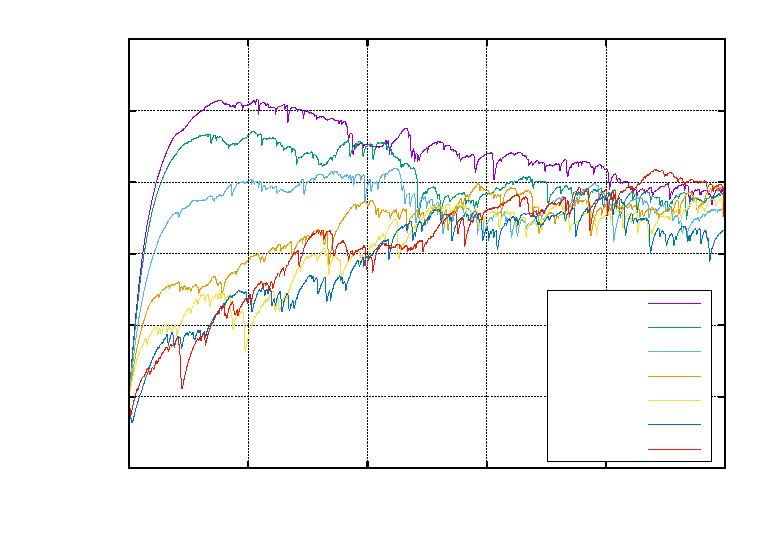
\includegraphics[width={360.00bp},height={252.00bp}]{./Contrainte-Deformation}}%
    \gplfronttext
  \end{picture}%
\endgroup
}
        \caption{Déformation Volumique}
        \label{fig:defvol}
    \end{subfigure}
    \hfill
    \begin{subfigure}[b]{0.49\textwidth}
        \centering \small
        \scalebox{0.5}{% GNUPLOT: LaTeX picture with Postscript
\begingroup
  \makeatletter
  \providecommand\color[2][]{%
    \GenericError{(gnuplot) \space\space\space\@spaces}{%
      Package color not loaded in conjunction with
      terminal option `colourtext'%
    }{See the gnuplot documentation for explanation.%
    }{Either use 'blacktext' in gnuplot or load the package
      color.sty in LaTeX.}%
    \renewcommand\color[2][]{}%
  }%
  \providecommand\includegraphics[2][]{%
    \GenericError{(gnuplot) \space\space\space\@spaces}{%
      Package graphicx or graphics not loaded%
    }{See the gnuplot documentation for explanation.%
    }{The gnuplot epslatex terminal needs graphicx.sty or graphics.sty.}%
    \renewcommand\includegraphics[2][]{}%
  }%
  \providecommand\rotatebox[2]{#2}%
  \@ifundefined{ifGPcolor}{%
    \newif\ifGPcolor
    \GPcolortrue
  }{}%
  \@ifundefined{ifGPblacktext}{%
    \newif\ifGPblacktext
    \GPblacktexttrue
  }{}%
  % define a \g@addto@macro without @ in the name:
  \let\gplgaddtomacro\g@addto@macro
  % define empty templates for all commands taking text:
  \gdef\gplbacktext{}%
  \gdef\gplfronttext{}%
  \makeatother
  \ifGPblacktext
    % no textcolor at all
    \def\colorrgb#1{}%
    \def\colorgray#1{}%
  \else
    % gray or color?
    \ifGPcolor
      \def\colorrgb#1{\color[rgb]{#1}}%
      \def\colorgray#1{\color[gray]{#1}}%
      \expandafter\def\csname LTw\endcsname{\color{white}}%
      \expandafter\def\csname LTb\endcsname{\color{black}}%
      \expandafter\def\csname LTa\endcsname{\color{black}}%
      \expandafter\def\csname LT0\endcsname{\color[rgb]{1,0,0}}%
      \expandafter\def\csname LT1\endcsname{\color[rgb]{0,1,0}}%
      \expandafter\def\csname LT2\endcsname{\color[rgb]{0,0,1}}%
      \expandafter\def\csname LT3\endcsname{\color[rgb]{1,0,1}}%
      \expandafter\def\csname LT4\endcsname{\color[rgb]{0,1,1}}%
      \expandafter\def\csname LT5\endcsname{\color[rgb]{1,1,0}}%
      \expandafter\def\csname LT6\endcsname{\color[rgb]{0,0,0}}%
      \expandafter\def\csname LT7\endcsname{\color[rgb]{1,0.3,0}}%
      \expandafter\def\csname LT8\endcsname{\color[rgb]{0.5,0.5,0.5}}%
    \else
      % gray
      \def\colorrgb#1{\color{black}}%
      \def\colorgray#1{\color[gray]{#1}}%
      \expandafter\def\csname LTw\endcsname{\color{white}}%
      \expandafter\def\csname LTb\endcsname{\color{black}}%
      \expandafter\def\csname LTa\endcsname{\color{black}}%
      \expandafter\def\csname LT0\endcsname{\color{black}}%
      \expandafter\def\csname LT1\endcsname{\color{black}}%
      \expandafter\def\csname LT2\endcsname{\color{black}}%
      \expandafter\def\csname LT3\endcsname{\color{black}}%
      \expandafter\def\csname LT4\endcsname{\color{black}}%
      \expandafter\def\csname LT5\endcsname{\color{black}}%
      \expandafter\def\csname LT6\endcsname{\color{black}}%
      \expandafter\def\csname LT7\endcsname{\color{black}}%
      \expandafter\def\csname LT8\endcsname{\color{black}}%
    \fi
  \fi
    \setlength{\unitlength}{0.0500bp}%
    \ifx\gptboxheight\undefined%
      \newlength{\gptboxheight}%
      \newlength{\gptboxwidth}%
      \newsavebox{\gptboxtext}%
    \fi%
    \setlength{\fboxrule}{0.5pt}%
    \setlength{\fboxsep}{1pt}%
    \definecolor{tbcol}{rgb}{1,1,1}%
\begin{picture}(7200.00,5040.00)%
    \gplgaddtomacro\gplbacktext{%
      \csname LTb\endcsname%%
      \put(682,704){\makebox(0,0)[r]{\strut{}$-4$}}%
      \csname LTb\endcsname%%
      \put(682,1161){\makebox(0,0)[r]{\strut{}$-3$}}%
      \csname LTb\endcsname%%
      \put(682,1618){\makebox(0,0)[r]{\strut{}$-2$}}%
      \csname LTb\endcsname%%
      \put(682,2076){\makebox(0,0)[r]{\strut{}$-1$}}%
      \csname LTb\endcsname%%
      \put(682,2533){\makebox(0,0)[r]{\strut{}$0$}}%
      \csname LTb\endcsname%%
      \put(682,2990){\makebox(0,0)[r]{\strut{}$1$}}%
      \csname LTb\endcsname%%
      \put(682,3447){\makebox(0,0)[r]{\strut{}$2$}}%
      \csname LTb\endcsname%%
      \put(682,3905){\makebox(0,0)[r]{\strut{}$3$}}%
      \csname LTb\endcsname%%
      \put(682,4362){\makebox(0,0)[r]{\strut{}$4$}}%
      \csname LTb\endcsname%%
      \put(682,4819){\makebox(0,0)[r]{\strut{}$5$}}%
      \csname LTb\endcsname%%
      \put(814,484){\makebox(0,0){\strut{}$0$}}%
      \csname LTb\endcsname%%
      \put(2012,484){\makebox(0,0){\strut{}$2$}}%
      \csname LTb\endcsname%%
      \put(3210,484){\makebox(0,0){\strut{}$4$}}%
      \csname LTb\endcsname%%
      \put(4407,484){\makebox(0,0){\strut{}$6$}}%
      \csname LTb\endcsname%%
      \put(5605,484){\makebox(0,0){\strut{}$8$}}%
      \csname LTb\endcsname%%
      \put(6803,484){\makebox(0,0){\strut{}$10$}}%
    }%
    \gplgaddtomacro\gplfronttext{%
      \csname LTb\endcsname%%
      \put(209,2761){\rotatebox{-270}{\makebox(0,0){\strut{}$\varepsilon_{v}$ (\%)}}}%
      \put(3808,154){\makebox(0,0){\strut{}$\varepsilon_{yy}$ (\%)}}%
      \csname LTb\endcsname%%
      \put(1810,4639){\makebox(0,0)[r]{\strut{}$\mu = 0$}}%
      \csname LTb\endcsname%%
      \put(1810,4405){\makebox(0,0)[r]{\strut{}$\mu = 0.1$}}%
      \csname LTb\endcsname%%
      \put(1810,4171){\makebox(0,0)[r]{\strut{}$\mu = 0.2$}}%
      \csname LTb\endcsname%%
      \put(1810,3937){\makebox(0,0)[r]{\strut{}$\mu = 0.3$}}%
      \csname LTb\endcsname%%
      \put(1810,3703){\makebox(0,0)[r]{\strut{}$\mu = 0.4$}}%
      \csname LTb\endcsname%%
      \put(1810,3469){\makebox(0,0)[r]{\strut{}$\mu = 0.45$}}%
      \csname LTb\endcsname%%
      \put(1810,3235){\makebox(0,0)[r]{\strut{}$\mu = 0.5$}}%
    }%
    \gplbacktext
    \put(0,0){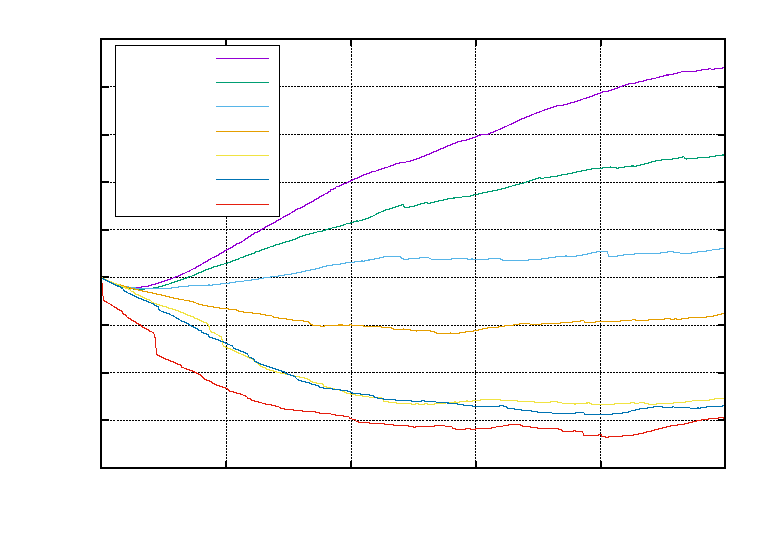
\includegraphics[width={360.00bp},height={252.00bp}]{./Deformation_Volumique}}%
    \gplfronttext
  \end{picture}%
\endgroup
}
        \caption{Courbe Contrainte-Déformation}
        \label{fig:contrainte}
    \end{subfigure}
    \caption{Comparaison des réponses}
    \label{fig:comparaison}
\end{figure}

\begin{equation}
    \frac{q}{p} \approx \frac{\sigma_{yy} - \frac{1}{2} (\sigma_{xx} + \sigma_{zz})}{\frac{1}{2} (\sigma_{xx} + \sigma_{zz})}
\end{equation}

Dans la section 1 de ce chapitre, nous avons effectué une compression isotrope et créé des échantillons avec des contraintes internes égales dans les deux sens. A partir de là, on voit l'effet du coefficient de frottement sur les comportements du materiau granulaire comme Ncontact, Z et e et et les limites de ce que nous pouvons réaliser.
Dans chapitre 2, nous pouvons voir qu’avec la différente valeur de $\mu$ dans compression isotrope, nous obtiendrons l’échantillons avec différent compacité donc ils se comportent de manière très différente.
Concernant la contrainte, le pic augmente avec la compacité du VE. Un VE très lâche ne présente pas de pic. Pour des grandes déformations, tous les échantillons tendent vers un même palier (l’état critique).
Ces simulations confirment alors la théorie de l’état critique: Une fois l’état critique est atteint, la déformation plastique peut augmenter infiniment, à une contrainte déviatorique constante. Les échantillons denses représentent des comportements contractants et puis dilatants, alors que ceux des échantillons lâches sont purement contractants.
\paragraph{La force entre les grains}
\begin{figure}[h!]
    \centering
    \subfloat[norme des forces]{\scalebox{0.33}{\small % GNUPLOT: LaTeX picture with Postscript
\begingroup
  \makeatletter
  \providecommand\color[2][]{%
    \GenericError{(gnuplot) \space\space\space\@spaces}{%
      Package color not loaded in conjunction with
      terminal option `colourtext'%
    }{See the gnuplot documentation for explanation.%
    }{Either use 'blacktext' in gnuplot or load the package
      color.sty in LaTeX.}%
    \renewcommand\color[2][]{}%
  }%
  \providecommand\includegraphics[2][]{%
    \GenericError{(gnuplot) \space\space\space\@spaces}{%
      Package graphicx or graphics not loaded%
    }{See the gnuplot documentation for explanation.%
    }{The gnuplot epslatex terminal needs graphicx.sty or graphics.sty.}%
    \renewcommand\includegraphics[2][]{}%
  }%
  \providecommand\rotatebox[2]{#2}%
  \@ifundefined{ifGPcolor}{%
    \newif\ifGPcolor
    \GPcolortrue
  }{}%
  \@ifundefined{ifGPblacktext}{%
    \newif\ifGPblacktext
    \GPblacktexttrue
  }{}%
  % define a \g@addto@macro without @ in the name:
  \let\gplgaddtomacro\g@addto@macro
  % define empty templates for all commands taking text:
  \gdef\gplbacktext{}%
  \gdef\gplfronttext{}%
  \makeatother
  \ifGPblacktext
    % no textcolor at all
    \def\colorrgb#1{}%
    \def\colorgray#1{}%
  \else
    % gray or color?
    \ifGPcolor
      \def\colorrgb#1{\color[rgb]{#1}}%
      \def\colorgray#1{\color[gray]{#1}}%
      \expandafter\def\csname LTw\endcsname{\color{white}}%
      \expandafter\def\csname LTb\endcsname{\color{black}}%
      \expandafter\def\csname LTa\endcsname{\color{black}}%
      \expandafter\def\csname LT0\endcsname{\color[rgb]{1,0,0}}%
      \expandafter\def\csname LT1\endcsname{\color[rgb]{0,1,0}}%
      \expandafter\def\csname LT2\endcsname{\color[rgb]{0,0,1}}%
      \expandafter\def\csname LT3\endcsname{\color[rgb]{1,0,1}}%
      \expandafter\def\csname LT4\endcsname{\color[rgb]{0,1,1}}%
      \expandafter\def\csname LT5\endcsname{\color[rgb]{1,1,0}}%
      \expandafter\def\csname LT6\endcsname{\color[rgb]{0,0,0}}%
      \expandafter\def\csname LT7\endcsname{\color[rgb]{1,0.3,0}}%
      \expandafter\def\csname LT8\endcsname{\color[rgb]{0.5,0.5,0.5}}%
    \else
      % gray
      \def\colorrgb#1{\color{black}}%
      \def\colorgray#1{\color[gray]{#1}}%
      \expandafter\def\csname LTw\endcsname{\color{white}}%
      \expandafter\def\csname LTb\endcsname{\color{black}}%
      \expandafter\def\csname LTa\endcsname{\color{black}}%
      \expandafter\def\csname LT0\endcsname{\color{black}}%
      \expandafter\def\csname LT1\endcsname{\color{black}}%
      \expandafter\def\csname LT2\endcsname{\color{black}}%
      \expandafter\def\csname LT3\endcsname{\color{black}}%
      \expandafter\def\csname LT4\endcsname{\color{black}}%
      \expandafter\def\csname LT5\endcsname{\color{black}}%
      \expandafter\def\csname LT6\endcsname{\color{black}}%
      \expandafter\def\csname LT7\endcsname{\color{black}}%
      \expandafter\def\csname LT8\endcsname{\color{black}}%
    \fi
  \fi
    \setlength{\unitlength}{0.0500bp}%
    \ifx\gptboxheight\undefined%
      \newlength{\gptboxheight}%
      \newlength{\gptboxwidth}%
      \newsavebox{\gptboxtext}%
    \fi%
    \setlength{\fboxrule}{0.5pt}%
    \setlength{\fboxsep}{1pt}%
    \definecolor{tbcol}{rgb}{1,1,1}%
\begin{picture}(7200.00,5040.00)%
    \gplgaddtomacro\gplbacktext{%
      \csname LTb\endcsname%%
      \put(946,704){\makebox(0,0)[r]{\strut{}$0.05$}}%
      \csname LTb\endcsname%%
      \put(946,1390){\makebox(0,0)[r]{\strut{}$0.1$}}%
      \csname LTb\endcsname%%
      \put(946,2076){\makebox(0,0)[r]{\strut{}$0.15$}}%
      \csname LTb\endcsname%%
      \put(946,2762){\makebox(0,0)[r]{\strut{}$0.2$}}%
      \csname LTb\endcsname%%
      \put(946,3447){\makebox(0,0)[r]{\strut{}$0.25$}}%
      \csname LTb\endcsname%%
      \put(946,4133){\makebox(0,0)[r]{\strut{}$0.3$}}%
      \csname LTb\endcsname%%
      \put(946,4819){\makebox(0,0)[r]{\strut{}$0.35$}}%
      \csname LTb\endcsname%%
      \put(1078,484){\makebox(0,0){\strut{}$0$}}%
      \csname LTb\endcsname%%
      \put(2223,484){\makebox(0,0){\strut{}$2$}}%
      \csname LTb\endcsname%%
      \put(3368,484){\makebox(0,0){\strut{}$4$}}%
      \csname LTb\endcsname%%
      \put(4513,484){\makebox(0,0){\strut{}$6$}}%
      \csname LTb\endcsname%%
      \put(5658,484){\makebox(0,0){\strut{}$8$}}%
      \csname LTb\endcsname%%
      \put(6803,484){\makebox(0,0){\strut{}$10$}}%
    }%
    \gplgaddtomacro\gplfronttext{%
      \csname LTb\endcsname%%
      \put(209,2761){\rotatebox{-270}{\makebox(0,0){\strut{}$\langle\frac{f_t}{f_n}\rangle$}}}%
      \put(3940,154){\makebox(0,0){\strut{}$\varepsilon_{yy}$ (\%)}}%
      \csname LTb\endcsname%%
      \put(5960,2054){\makebox(0,0)[r]{\strut{}$\mu = 0$}}%
      \csname LTb\endcsname%%
      \put(5960,1820){\makebox(0,0)[r]{\strut{}$\mu = 0.1$}}%
      \csname LTb\endcsname%%
      \put(5960,1586){\makebox(0,0)[r]{\strut{}$\mu = 0.2$}}%
      \csname LTb\endcsname%%
      \put(5960,1352){\makebox(0,0)[r]{\strut{}$\mu = 0.3$}}%
      \csname LTb\endcsname%%
      \put(5960,1118){\makebox(0,0)[r]{\strut{}$\mu = 0.4$}}%
      \csname LTb\endcsname%%
      \put(5960,884){\makebox(0,0)[r]{\strut{}$\mu = 0.5$}}%
    }%
    \gplbacktext
    \put(0,0){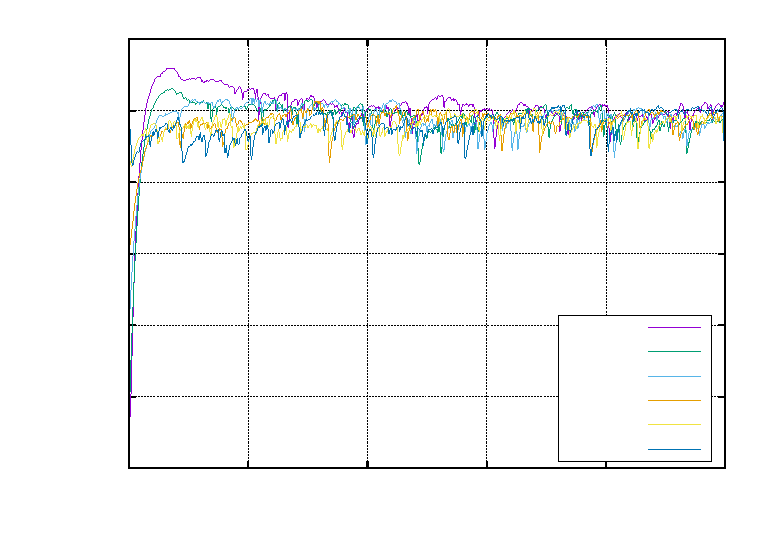
\includegraphics[width={360.00bp},height={252.00bp}]{./Taux_ft_fn}}%
    \gplfronttext
  \end{picture}%
\endgroup
}\label{fig:palier_a}}
    \subfloat[L’indice de vide]{\scalebox{0.33}{\small % GNUPLOT: LaTeX picture with Postscript
\begingroup
  \makeatletter
  \providecommand\color[2][]{%
    \GenericError{(gnuplot) \space\space\space\@spaces}{%
      Package color not loaded in conjunction with
      terminal option `colourtext'%
    }{See the gnuplot documentation for explanation.%
    }{Either use 'blacktext' in gnuplot or load the package
      color.sty in LaTeX.}%
    \renewcommand\color[2][]{}%
  }%
  \providecommand\includegraphics[2][]{%
    \GenericError{(gnuplot) \space\space\space\@spaces}{%
      Package graphicx or graphics not loaded%
    }{See the gnuplot documentation for explanation.%
    }{The gnuplot epslatex terminal needs graphicx.sty or graphics.sty.}%
    \renewcommand\includegraphics[2][]{}%
  }%
  \providecommand\rotatebox[2]{#2}%
  \@ifundefined{ifGPcolor}{%
    \newif\ifGPcolor
    \GPcolortrue
  }{}%
  \@ifundefined{ifGPblacktext}{%
    \newif\ifGPblacktext
    \GPblacktextfalse
  }{}%
  % define a \g@addto@macro without @ in the name:
  \let\gplgaddtomacro\g@addto@macro
  % define empty templates for all commands taking text:
  \gdef\gplbacktext{}%
  \gdef\gplfronttext{}%
  \makeatother
  \ifGPblacktext
    % no textcolor at all
    \def\colorrgb#1{}%
    \def\colorgray#1{}%
  \else
    % gray or color?
    \ifGPcolor
      \def\colorrgb#1{\color[rgb]{#1}}%
      \def\colorgray#1{\color[gray]{#1}}%
      \expandafter\def\csname LTw\endcsname{\color{white}}%
      \expandafter\def\csname LTb\endcsname{\color{black}}%
      \expandafter\def\csname LTa\endcsname{\color{black}}%
      \expandafter\def\csname LT0\endcsname{\color[rgb]{1,0,0}}%
      \expandafter\def\csname LT1\endcsname{\color[rgb]{0,1,0}}%
      \expandafter\def\csname LT2\endcsname{\color[rgb]{0,0,1}}%
      \expandafter\def\csname LT3\endcsname{\color[rgb]{1,0,1}}%
      \expandafter\def\csname LT4\endcsname{\color[rgb]{0,1,1}}%
      \expandafter\def\csname LT5\endcsname{\color[rgb]{1,1,0}}%
      \expandafter\def\csname LT6\endcsname{\color[rgb]{0,0,0}}%
      \expandafter\def\csname LT7\endcsname{\color[rgb]{1,0.3,0}}%
      \expandafter\def\csname LT8\endcsname{\color[rgb]{0.5,0.5,0.5}}%
    \else
      % gray
      \def\colorrgb#1{\color{black}}%
      \def\colorgray#1{\color[gray]{#1}}%
      \expandafter\def\csname LTw\endcsname{\color{white}}%
      \expandafter\def\csname LTb\endcsname{\color{black}}%
      \expandafter\def\csname LTa\endcsname{\color{black}}%
      \expandafter\def\csname LT0\endcsname{\color{black}}%
      \expandafter\def\csname LT1\endcsname{\color{black}}%
      \expandafter\def\csname LT2\endcsname{\color{black}}%
      \expandafter\def\csname LT3\endcsname{\color{black}}%
      \expandafter\def\csname LT4\endcsname{\color{black}}%
      \expandafter\def\csname LT5\endcsname{\color{black}}%
      \expandafter\def\csname LT6\endcsname{\color{black}}%
      \expandafter\def\csname LT7\endcsname{\color{black}}%
      \expandafter\def\csname LT8\endcsname{\color{black}}%
    \fi
  \fi
    \setlength{\unitlength}{0.0500bp}%
    \ifx\gptboxheight\undefined%
      \newlength{\gptboxheight}%
      \newlength{\gptboxwidth}%
      \newsavebox{\gptboxtext}%
    \fi%
    \setlength{\fboxrule}{0.5pt}%
    \setlength{\fboxsep}{1pt}%
    \definecolor{tbcol}{rgb}{1,1,1}%
\begin{picture}(7200.00,5040.00)%
    \gplgaddtomacro\gplbacktext{%
      \csname LTb\endcsname%%
      \put(946,1834){\makebox(0,0)[r]{\strut{}$0.62$}}%
      \csname LTb\endcsname%%
      \put(946,2293){\makebox(0,0)[r]{\strut{}$0.64$}}%
      \csname LTb\endcsname%%
      \put(946,2752){\makebox(0,0)[r]{\strut{}$0.66$}}%
      \csname LTb\endcsname%%
      \put(946,3212){\makebox(0,0)[r]{\strut{}$0.68$}}%
      \csname LTb\endcsname%%
      \put(946,3671){\makebox(0,0)[r]{\strut{}$0.7$}}%
      \csname LTb\endcsname%%
      \put(946,4130){\makebox(0,0)[r]{\strut{}$0.72$}}%
      \csname LTb\endcsname%%
      \put(946,4589){\makebox(0,0)[r]{\strut{}$0.74$}}%
      \csname LTb\endcsname%%
      \put(1078,1384){\makebox(0,0){\strut{}$0$}}%
      \csname LTb\endcsname%%
      \put(2223,1384){\makebox(0,0){\strut{}$20$}}%
      \csname LTb\endcsname%%
      \put(3368,1384){\makebox(0,0){\strut{}$40$}}%
      \csname LTb\endcsname%%
      \put(4513,1384){\makebox(0,0){\strut{}$60$}}%
      \csname LTb\endcsname%%
      \put(5658,1384){\makebox(0,0){\strut{}$80$}}%
      \csname LTb\endcsname%%
      \put(6803,1384){\makebox(0,0){\strut{}$100$}}%
    }%
    \gplgaddtomacro\gplfronttext{%
      \csname LTb\endcsname%%
      \put(209,3211){\rotatebox{-270}{\makebox(0,0){\strut{}e}}}%
      \put(3940,1054){\makebox(0,0){\strut{}$\varepsilon_{yy}$ (\%)}}%
      \csname LTb\endcsname%%
      \put(2046,813){\makebox(0,0)[r]{\strut{}$I = 1 \times 10^{-4}$}}%
      \csname LTb\endcsname%%
      \put(2046,513){\makebox(0,0)[r]{\strut{}$I = 1 \times 10^{-3}$}}%
      \csname LTb\endcsname%%
      \put(2046,213){\makebox(0,0)[r]{\strut{}$I = 2 \times 10^{-3}$}}%
      \csname LTb\endcsname%%
      \put(4269,813){\makebox(0,0)[r]{\strut{}$I = 4 \times 10^{-3}$}}%
      \csname LTb\endcsname%%
      \put(4269,513){\makebox(0,0)[r]{\strut{}$I = 6 \times 10^{-3}$}}%
      \csname LTb\endcsname%%
      \put(4269,213){\makebox(0,0)[r]{\strut{}$I = 8 \times 10^{-3}$}}%
      \csname LTb\endcsname%%
      \put(6492,813){\makebox(0,0)[r]{\strut{}$I = 1 \times 10^{-2}$}}%
    }%
    \gplbacktext
    \put(0,0){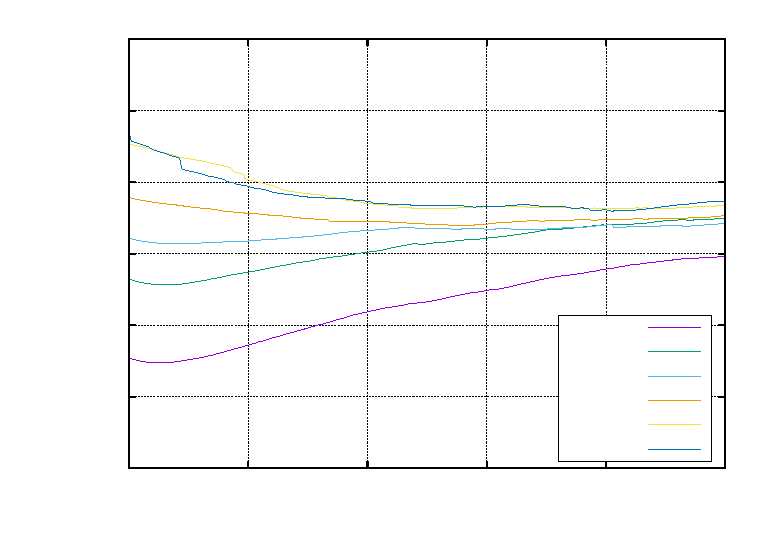
\includegraphics[width={360.00bp},height={252.00bp}]{./RapportVides}}%
    \gplfronttext
  \end{picture}%
\endgroup
}\label{fig:palier_b}}
    \subfloat[Nombre de Contact]{\scalebox{0.33}{\small % GNUPLOT: LaTeX picture with Postscript
\begingroup
  \makeatletter
  \providecommand\color[2][]{%
    \GenericError{(gnuplot) \space\space\space\@spaces}{%
      Package color not loaded in conjunction with
      terminal option `colourtext'%
    }{See the gnuplot documentation for explanation.%
    }{Either use 'blacktext' in gnuplot or load the package
      color.sty in LaTeX.}%
    \renewcommand\color[2][]{}%
  }%
  \providecommand\includegraphics[2][]{%
    \GenericError{(gnuplot) \space\space\space\@spaces}{%
      Package graphicx or graphics not loaded%
    }{See the gnuplot documentation for explanation.%
    }{The gnuplot epslatex terminal needs graphicx.sty or graphics.sty.}%
    \renewcommand\includegraphics[2][]{}%
  }%
  \providecommand\rotatebox[2]{#2}%
  \@ifundefined{ifGPcolor}{%
    \newif\ifGPcolor
    \GPcolortrue
  }{}%
  \@ifundefined{ifGPblacktext}{%
    \newif\ifGPblacktext
    \GPblacktexttrue
  }{}%
  % define a \g@addto@macro without @ in the name:
  \let\gplgaddtomacro\g@addto@macro
  % define empty templates for all commands taking text:
  \gdef\gplbacktext{}%
  \gdef\gplfronttext{}%
  \makeatother
  \ifGPblacktext
    % no textcolor at all
    \def\colorrgb#1{}%
    \def\colorgray#1{}%
  \else
    % gray or color?
    \ifGPcolor
      \def\colorrgb#1{\color[rgb]{#1}}%
      \def\colorgray#1{\color[gray]{#1}}%
      \expandafter\def\csname LTw\endcsname{\color{white}}%
      \expandafter\def\csname LTb\endcsname{\color{black}}%
      \expandafter\def\csname LTa\endcsname{\color{black}}%
      \expandafter\def\csname LT0\endcsname{\color[rgb]{1,0,0}}%
      \expandafter\def\csname LT1\endcsname{\color[rgb]{0,1,0}}%
      \expandafter\def\csname LT2\endcsname{\color[rgb]{0,0,1}}%
      \expandafter\def\csname LT3\endcsname{\color[rgb]{1,0,1}}%
      \expandafter\def\csname LT4\endcsname{\color[rgb]{0,1,1}}%
      \expandafter\def\csname LT5\endcsname{\color[rgb]{1,1,0}}%
      \expandafter\def\csname LT6\endcsname{\color[rgb]{0,0,0}}%
      \expandafter\def\csname LT7\endcsname{\color[rgb]{1,0.3,0}}%
      \expandafter\def\csname LT8\endcsname{\color[rgb]{0.5,0.5,0.5}}%
    \else
      % gray
      \def\colorrgb#1{\color{black}}%
      \def\colorgray#1{\color[gray]{#1}}%
      \expandafter\def\csname LTw\endcsname{\color{white}}%
      \expandafter\def\csname LTb\endcsname{\color{black}}%
      \expandafter\def\csname LTa\endcsname{\color{black}}%
      \expandafter\def\csname LT0\endcsname{\color{black}}%
      \expandafter\def\csname LT1\endcsname{\color{black}}%
      \expandafter\def\csname LT2\endcsname{\color{black}}%
      \expandafter\def\csname LT3\endcsname{\color{black}}%
      \expandafter\def\csname LT4\endcsname{\color{black}}%
      \expandafter\def\csname LT5\endcsname{\color{black}}%
      \expandafter\def\csname LT6\endcsname{\color{black}}%
      \expandafter\def\csname LT7\endcsname{\color{black}}%
      \expandafter\def\csname LT8\endcsname{\color{black}}%
    \fi
  \fi
    \setlength{\unitlength}{0.0500bp}%
    \ifx\gptboxheight\undefined%
      \newlength{\gptboxheight}%
      \newlength{\gptboxwidth}%
      \newsavebox{\gptboxtext}%
    \fi%
    \setlength{\fboxrule}{0.5pt}%
    \setlength{\fboxsep}{1pt}%
    \definecolor{tbcol}{rgb}{1,1,1}%
\begin{picture}(7200.00,5040.00)%
    \gplgaddtomacro\gplbacktext{%
      \csname LTb\endcsname%%
      \put(814,704){\makebox(0,0)[r]{\strut{}$2$}}%
      \csname LTb\endcsname%%
      \put(814,1527){\makebox(0,0)[r]{\strut{}$2.2$}}%
      \csname LTb\endcsname%%
      \put(814,2350){\makebox(0,0)[r]{\strut{}$2.4$}}%
      \csname LTb\endcsname%%
      \put(814,3173){\makebox(0,0)[r]{\strut{}$2.6$}}%
      \csname LTb\endcsname%%
      \put(814,3996){\makebox(0,0)[r]{\strut{}$2.8$}}%
      \csname LTb\endcsname%%
      \put(814,4819){\makebox(0,0)[r]{\strut{}$3$}}%
      \csname LTb\endcsname%%
      \put(946,484){\makebox(0,0){\strut{}$0$}}%
      \csname LTb\endcsname%%
      \put(2117,484){\makebox(0,0){\strut{}$2$}}%
      \csname LTb\endcsname%%
      \put(3289,484){\makebox(0,0){\strut{}$4$}}%
      \csname LTb\endcsname%%
      \put(4460,484){\makebox(0,0){\strut{}$6$}}%
      \csname LTb\endcsname%%
      \put(5632,484){\makebox(0,0){\strut{}$8$}}%
      \csname LTb\endcsname%%
      \put(6803,484){\makebox(0,0){\strut{}$10$}}%
    }%
    \gplgaddtomacro\gplfronttext{%
      \csname LTb\endcsname%%
      \put(209,2761){\rotatebox{-270}{\makebox(0,0){\strut{}$N_{contacts}/N_{particules}$}}}%
      \put(3874,154){\makebox(0,0){\strut{}$\varepsilon_{yy}$ (\%)}}%
      \csname LTb\endcsname%%
      \put(5960,4639){\makebox(0,0)[r]{\strut{}$\mu = 0$}}%
      \csname LTb\endcsname%%
      \put(5960,4405){\makebox(0,0)[r]{\strut{}$\mu = 0.1$}}%
      \csname LTb\endcsname%%
      \put(5960,4171){\makebox(0,0)[r]{\strut{}$\mu = 0.2$}}%
      \csname LTb\endcsname%%
      \put(5960,3937){\makebox(0,0)[r]{\strut{}$\mu = 0.3$}}%
      \csname LTb\endcsname%%
      \put(5960,3703){\makebox(0,0)[r]{\strut{}$\mu = 0.4$}}%
      \csname LTb\endcsname%%
      \put(5960,3469){\makebox(0,0)[r]{\strut{}$\mu = 0.5$}}%
    }%
    \gplbacktext
    \put(0,0){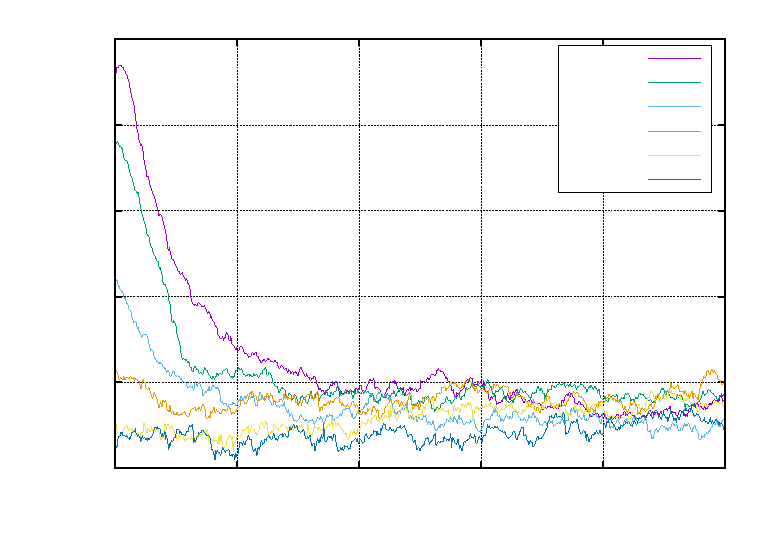
\includegraphics[width={360.00bp},height={252.00bp}]{./NombreContacts}}%
    \gplfronttext
  \end{picture}%
\endgroup
}\label{fig:palier_c}}
  \caption{Palier}
    \label{fig:Palier}
\end{figure}
Quand la déformation est suffisamment grande (environ 8 \%), les courbes tendent progressivement vers un même palier déterminé.

\subsubsection{Cercle de Mohr}
\begin{figure}[h!]
    \centering
    \begin{subfigure}[b]{0.48\textwidth}
        \centering
        \scalebox{0.6}{\small % GNUPLOT: LaTeX picture with Postscript
\begingroup
  \makeatletter
  \providecommand\color[2][]{%
    \GenericError{(gnuplot) \space\space\space\@spaces}{%
      Package color not loaded in conjunction with
      terminal option `colourtext'%
    }{See the gnuplot documentation for explanation.%
    }{Either use 'blacktext' in gnuplot or load the package
      color.sty in LaTeX.}%
    \renewcommand\color[2][]{}%
  }%
  \providecommand\includegraphics[2][]{%
    \GenericError{(gnuplot) \space\space\space\@spaces}{%
      Package graphicx or graphics not loaded%
    }{See the gnuplot documentation for explanation.%
    }{The gnuplot epslatex terminal needs graphicx.sty or graphics.sty.}%
    \renewcommand\includegraphics[2][]{}%
  }%
  \providecommand\rotatebox[2]{#2}%
  \@ifundefined{ifGPcolor}{%
    \newif\ifGPcolor
    \GPcolortrue
  }{}%
  \@ifundefined{ifGPblacktext}{%
    \newif\ifGPblacktext
    \GPblacktextfalse
  }{}%
  % define a \g@addto@macro without @ in the name:
  \let\gplgaddtomacro\g@addto@macro
  % define empty templates for all commands taking text:
  \gdef\gplbacktext{}%
  \gdef\gplfronttext{}%
  \makeatother
  \ifGPblacktext
    % no textcolor at all
    \def\colorrgb#1{}%
    \def\colorgray#1{}%
  \else
    % gray or color?
    \ifGPcolor
      \def\colorrgb#1{\color[rgb]{#1}}%
      \def\colorgray#1{\color[gray]{#1}}%
      \expandafter\def\csname LTw\endcsname{\color{white}}%
      \expandafter\def\csname LTb\endcsname{\color{black}}%
      \expandafter\def\csname LTa\endcsname{\color{black}}%
      \expandafter\def\csname LT0\endcsname{\color[rgb]{1,0,0}}%
      \expandafter\def\csname LT1\endcsname{\color[rgb]{0,1,0}}%
      \expandafter\def\csname LT2\endcsname{\color[rgb]{0,0,1}}%
      \expandafter\def\csname LT3\endcsname{\color[rgb]{1,0,1}}%
      \expandafter\def\csname LT4\endcsname{\color[rgb]{0,1,1}}%
      \expandafter\def\csname LT5\endcsname{\color[rgb]{1,1,0}}%
      \expandafter\def\csname LT6\endcsname{\color[rgb]{0,0,0}}%
      \expandafter\def\csname LT7\endcsname{\color[rgb]{1,0.3,0}}%
      \expandafter\def\csname LT8\endcsname{\color[rgb]{0.5,0.5,0.5}}%
    \else
      % gray
      \def\colorrgb#1{\color{black}}%
      \def\colorgray#1{\color[gray]{#1}}%
      \expandafter\def\csname LTw\endcsname{\color{white}}%
      \expandafter\def\csname LTb\endcsname{\color{black}}%
      \expandafter\def\csname LTa\endcsname{\color{black}}%
      \expandafter\def\csname LT0\endcsname{\color{black}}%
      \expandafter\def\csname LT1\endcsname{\color{black}}%
      \expandafter\def\csname LT2\endcsname{\color{black}}%
      \expandafter\def\csname LT3\endcsname{\color{black}}%
      \expandafter\def\csname LT4\endcsname{\color{black}}%
      \expandafter\def\csname LT5\endcsname{\color{black}}%
      \expandafter\def\csname LT6\endcsname{\color{black}}%
      \expandafter\def\csname LT7\endcsname{\color{black}}%
      \expandafter\def\csname LT8\endcsname{\color{black}}%
    \fi
  \fi
    \setlength{\unitlength}{0.0500bp}%
    \ifx\gptboxheight\undefined%
      \newlength{\gptboxheight}%
      \newlength{\gptboxwidth}%
      \newsavebox{\gptboxtext}%
    \fi%
    \setlength{\fboxrule}{0.5pt}%
    \setlength{\fboxsep}{1pt}%
    \definecolor{tbcol}{rgb}{1,1,1}%
\begin{picture}(7200.00,5040.00)%
    \gplgaddtomacro\gplbacktext{%
      \csname LTb\endcsname%%
      \put(814,1785){\makebox(0,0)[r]{\strut{}$0$}}%
      \put(814,2273){\makebox(0,0)[r]{\strut{}$50$}}%
      \put(814,2762){\makebox(0,0)[r]{\strut{}$100$}}%
      \put(814,3250){\makebox(0,0)[r]{\strut{}$150$}}%
      \put(814,3738){\makebox(0,0)[r]{\strut{}$200$}}%
      \put(946,1565){\makebox(0,0){\strut{}$0$}}%
      \put(1922,1565){\makebox(0,0){\strut{}$100$}}%
      \put(2898,1565){\makebox(0,0){\strut{}$200$}}%
      \put(3875,1565){\makebox(0,0){\strut{}$300$}}%
      \put(4851,1565){\makebox(0,0){\strut{}$400$}}%
      \put(5827,1565){\makebox(0,0){\strut{}$500$}}%
      \put(6803,1565){\makebox(0,0){\strut{}$600$}}%
      \colorrgb{0.00,0.00,1.00}%%
      \put(6369,3409){\makebox(0,0)[l]{\strut{}$\varphi_1 = 17.36^\circ$}}%
      \colorrgb{1.00,0.00,0.00}%%
      \put(5149,3067){\makebox(0,0)[l]{\strut{}$\varphi_2 = \varphi_3 = 17.92^\circ$}}%
      \colorrgb{0.00,0.00,0.00}%%
      \put(3875,2957){\makebox(0,0){\strut{}\rotatebox{17}{$\tau= \sigma_n \times \tan(\varphi) + c$}}}%
    }%
    \gplgaddtomacro\gplfronttext{%
      \csname LTb\endcsname%%
      \put(209,2761){\rotatebox{-270}{\makebox(0,0){\strut{}$\tau$ (kPa)}}}%
      \put(3874,1235){\makebox(0,0){\strut{}$\sigma_n$ (kPa)}}%
    }%
    \gplbacktext
    \put(0,0){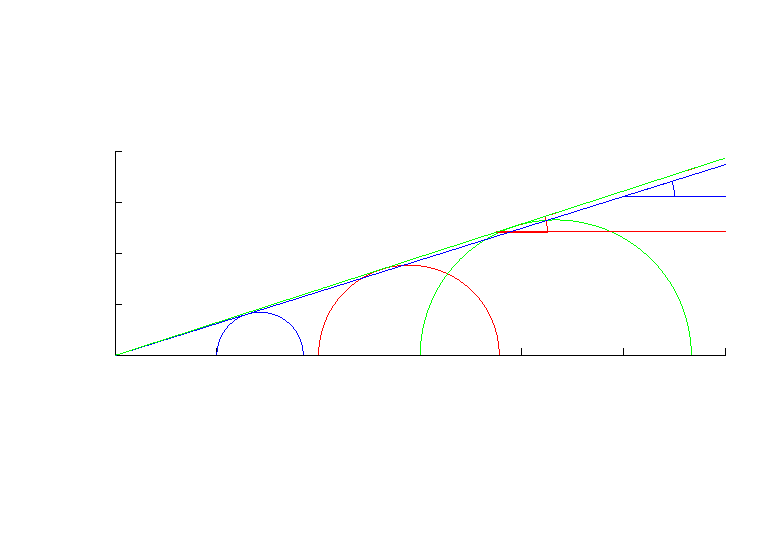
\includegraphics[width={360.00bp},height={252.00bp}]{CercleMohr}}%
    \gplfronttext
  \end{picture}%
\endgroup
}
        \caption{Dense}
        \label{fig:palier_a}
    \end{subfigure}
    \hfill
    \begin{subfigure}[b]{0.48\textwidth}
        \centering
        \scalebox{0.7}{\small % GNUPLOT: LaTeX picture with Postscript
\begingroup
  \makeatletter
  \providecommand\color[2][]{%
    \GenericError{(gnuplot) \space\space\space\@spaces}{%
      Package color not loaded in conjunction with
      terminal option `colourtext'%
    }{See the gnuplot documentation for explanation.%
    }{Either use 'blacktext' in gnuplot or load the package
      color.sty in LaTeX.}%
    \renewcommand\color[2][]{}%
  }%
  \providecommand\includegraphics[2][]{%
    \GenericError{(gnuplot) \space\space\space\@spaces}{%
      Package graphicx or graphics not loaded%
    }{See the gnuplot documentation for explanation.%
    }{The gnuplot epslatex terminal needs graphicx.sty or graphics.sty.}%
    \renewcommand\includegraphics[2][]{}%
  }%
  \providecommand\rotatebox[2]{#2}%
  \@ifundefined{ifGPcolor}{%
    \newif\ifGPcolor
    \GPcolortrue
  }{}%
  \@ifundefined{ifGPblacktext}{%
    \newif\ifGPblacktext
    \GPblacktextfalse
  }{}%
  % define a \g@addto@macro without @ in the name:
  \let\gplgaddtomacro\g@addto@macro
  % define empty templates for all commands taking text:
  \gdef\gplbacktext{}%
  \gdef\gplfronttext{}%
  \makeatother
  \ifGPblacktext
    % no textcolor at all
    \def\colorrgb#1{}%
    \def\colorgray#1{}%
  \else
    % gray or color?
    \ifGPcolor
      \def\colorrgb#1{\color[rgb]{#1}}%
      \def\colorgray#1{\color[gray]{#1}}%
      \expandafter\def\csname LTw\endcsname{\color{white}}%
      \expandafter\def\csname LTb\endcsname{\color{black}}%
      \expandafter\def\csname LTa\endcsname{\color{black}}%
      \expandafter\def\csname LT0\endcsname{\color[rgb]{1,0,0}}%
      \expandafter\def\csname LT1\endcsname{\color[rgb]{0,1,0}}%
      \expandafter\def\csname LT2\endcsname{\color[rgb]{0,0,1}}%
      \expandafter\def\csname LT3\endcsname{\color[rgb]{1,0,1}}%
      \expandafter\def\csname LT4\endcsname{\color[rgb]{0,1,1}}%
      \expandafter\def\csname LT5\endcsname{\color[rgb]{1,1,0}}%
      \expandafter\def\csname LT6\endcsname{\color[rgb]{0,0,0}}%
      \expandafter\def\csname LT7\endcsname{\color[rgb]{1,0.3,0}}%
      \expandafter\def\csname LT8\endcsname{\color[rgb]{0.5,0.5,0.5}}%
    \else
      % gray
      \def\colorrgb#1{\color{black}}%
      \def\colorgray#1{\color[gray]{#1}}%
      \expandafter\def\csname LTw\endcsname{\color{white}}%
      \expandafter\def\csname LTb\endcsname{\color{black}}%
      \expandafter\def\csname LTa\endcsname{\color{black}}%
      \expandafter\def\csname LT0\endcsname{\color{black}}%
      \expandafter\def\csname LT1\endcsname{\color{black}}%
      \expandafter\def\csname LT2\endcsname{\color{black}}%
      \expandafter\def\csname LT3\endcsname{\color{black}}%
      \expandafter\def\csname LT4\endcsname{\color{black}}%
      \expandafter\def\csname LT5\endcsname{\color{black}}%
      \expandafter\def\csname LT6\endcsname{\color{black}}%
      \expandafter\def\csname LT7\endcsname{\color{black}}%
      \expandafter\def\csname LT8\endcsname{\color{black}}%
    \fi
  \fi
    \setlength{\unitlength}{0.0500bp}%
    \ifx\gptboxheight\undefined%
      \newlength{\gptboxheight}%
      \newlength{\gptboxwidth}%
      \newsavebox{\gptboxtext}%
    \fi%
    \setlength{\fboxrule}{0.5pt}%
    \setlength{\fboxsep}{1pt}%
    \definecolor{tbcol}{rgb}{1,1,1}%
\begin{picture}(7200.00,5040.00)%
    \gplgaddtomacro\gplbacktext{%
      \csname LTb\endcsname%%
      \put(814,1942){\makebox(0,0)[r]{\strut{}$0$}}%
      \put(814,2176){\makebox(0,0)[r]{\strut{}$20$}}%
      \put(814,2410){\makebox(0,0)[r]{\strut{}$40$}}%
      \put(814,2644){\makebox(0,0)[r]{\strut{}$60$}}%
      \put(814,2879){\makebox(0,0)[r]{\strut{}$80$}}%
      \put(814,3113){\makebox(0,0)[r]{\strut{}$100$}}%
      \put(814,3347){\makebox(0,0)[r]{\strut{}$120$}}%
      \put(814,3581){\makebox(0,0)[r]{\strut{}$140$}}%
      \put(946,1722){\makebox(0,0){\strut{}$0$}}%
      \put(2117,1722){\makebox(0,0){\strut{}$100$}}%
      \put(3289,1722){\makebox(0,0){\strut{}$200$}}%
      \put(4460,1722){\makebox(0,0){\strut{}$300$}}%
      \put(5632,1722){\makebox(0,0){\strut{}$400$}}%
      \put(6803,1722){\makebox(0,0){\strut{}$500$}}%
      \colorrgb{0.00,0.00,1.00}%%
      \put(1649,2058){\makebox(0,0)[l]{\strut{}$\varphi_1 = 9.49^\circ$}}%
      \colorrgb{1.00,0.00,0.00}%%
      \put(3052,2130){\makebox(0,0)[l]{\strut{}$\varphi_2 = 10.24^\circ$}}%
      \colorrgb{0.00,1.00,0.00}%%
      \put(4498,2318){\makebox(0,0)[l]{\strut{}$\varphi_3 = 12.13^\circ$}}%
      \colorrgb{0.00,0.00,0.00}%%
      \put(3875,2843){\makebox(0,0){\strut{}\rotatebox{12}{$\tau= \sigma_n \times \tan(\varphi) + c$}}}%
    }%
    \gplgaddtomacro\gplfronttext{%
      \csname LTb\endcsname%%
      \put(209,2761){\rotatebox{-270}{\makebox(0,0){\strut{}$\tau$ (kPa)}}}%
      \put(3874,1392){\makebox(0,0){\strut{}$\sigma_n$ (kPa)}}%
    }%
    \gplbacktext
    \put(0,0){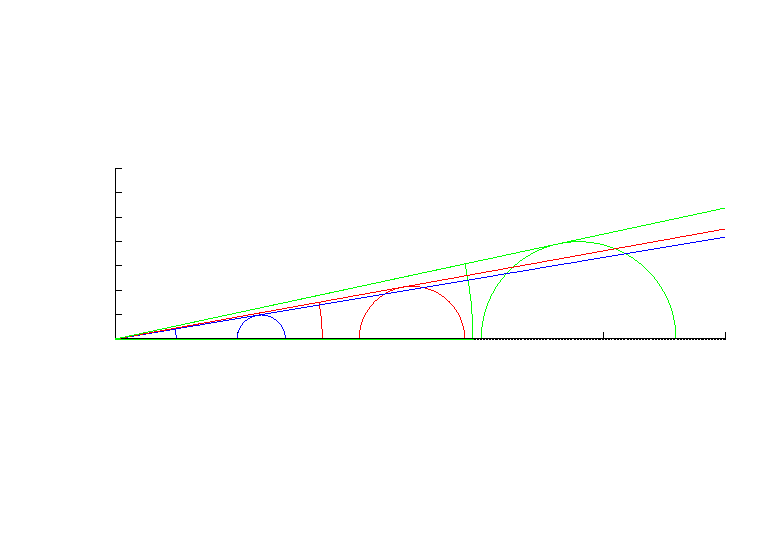
\includegraphics[width={360.00bp},height={252.00bp}]{LACHE_CercleMohr}}%
    \gplfronttext
  \end{picture}%
\endgroup
}
        \caption{Lâche}
        \label{fig:palier_b}
    \end{subfigure}
    \caption{Cercle du Mohr xanh do tim vang}
    \label{fig:CercleDuMohr}
\end{figure}
\subsubsection{Histoire du chargement}

\subsection{Recherche sur l'impact dynamique}

\subsubsection{Augmentation du nombre d'inertie (Montée la vitesse imposée)}
    \begin{table}
    \centering
    \begin{table}
    \centering
    \begin{tabular}{|c|c|c|c|}
    \hline
    \textbf{Symboles} & \textbf{Paramètres} & \textbf{Valeurs} & \textbf{Unité} \\ 
    \hline
    Nombre de particules & N & $15^3$ & -- \\  
    \hline
    Le rayon des particules & R & 0.003 $\div$ 0.005 & m \\  
    \hline
    Masse volumique & $\rho$  & 2500 & $\text{kg/m}^3$ \\
    \hline
    Contrainte isotrope & $\sigma_{xx} = \sigma_{zz}$ & 100, 200, 300 & kPa \\ 
    \hline
    Raideur normale et tangentielle & $k_n$ \& $k_t$ & \textcolor{black}{$3 \times 10^6$} & $\text{N/m}$ \\ 
    \hline
    Niveau de raideur & $\kappa$ & 1000 & -- \\ 
    \hline
    Coefficient de frottement & $\mu$ & 0.5 & -- \\ 
    \hline
    Déformation axiale & $\varepsilon_{\text{yy}}$ &  10 & $\%$ \\ 
    \hline
    Masse de la cellule périodique  & $h_{mass}$ &   \textcolor{black}{$7.13 \times 10^{-4}$}  & $\text{kg}$ \\ 
    \hline
    Nombre d’inertie & I & \textcolor{red}{$10^{-6}\  \& \ 10^{-2}$} & -- \\ 
    \hline
    Vitesse imposée & v & $10^{-3}\  \& \ 10 $ & m/s \\ 
    \hline
    Pas de temps & $d_t$  & $10^{-6}\  \& \ 10^{-10}$ & $\text{s}$\\
    \hline
    Coefficient d'amortissement & $\alpha$  & \textcolor{black}{$0.0 \ \& \ 0.7$} & --\\
    \hline
    \end{tabular}
    \caption{Valeurs des paramètres utilisés dans la compression triaxiale}
    \end{table}

\section{Couplage\ldots}

\chapter{Conclusion}

                                \begin{figure}
                                    \centering
                                  \small
                                  % GNUPLOT: LaTeX picture with Postscript
\begingroup
  \makeatletter
  \providecommand\color[2][]{%
    \GenericError{(gnuplot) \space\space\space\@spaces}{%
      Package color not loaded in conjunction with
      terminal option `colourtext'%
    }{See the gnuplot documentation for explanation.%
    }{Either use 'blacktext' in gnuplot or load the package
      color.sty in LaTeX.}%
    \renewcommand\color[2][]{}%
  }%
  \providecommand\includegraphics[2][]{%
    \GenericError{(gnuplot) \space\space\space\@spaces}{%
      Package graphicx or graphics not loaded%
    }{See the gnuplot documentation for explanation.%
    }{The gnuplot epslatex terminal needs graphicx.sty or graphics.sty.}%
    \renewcommand\includegraphics[2][]{}%
  }%
  \providecommand\rotatebox[2]{#2}%
  \@ifundefined{ifGPcolor}{%
    \newif\ifGPcolor
    \GPcolortrue
  }{}%
  \@ifundefined{ifGPblacktext}{%
    \newif\ifGPblacktext
    \GPblacktexttrue
  }{}%
  % define a \g@addto@macro without @ in the name:
  \let\gplgaddtomacro\g@addto@macro
  % define empty templates for all commands taking text:
  \gdef\gplbacktext{}%
  \gdef\gplfronttext{}%
  \makeatother
  \ifGPblacktext
    % no textcolor at all
    \def\colorrgb#1{}%
    \def\colorgray#1{}%
  \else
    % gray or color?
    \ifGPcolor
      \def\colorrgb#1{\color[rgb]{#1}}%
      \def\colorgray#1{\color[gray]{#1}}%
      \expandafter\def\csname LTw\endcsname{\color{white}}%
      \expandafter\def\csname LTb\endcsname{\color{black}}%
      \expandafter\def\csname LTa\endcsname{\color{black}}%
      \expandafter\def\csname LT0\endcsname{\color[rgb]{1,0,0}}%
      \expandafter\def\csname LT1\endcsname{\color[rgb]{0,1,0}}%
      \expandafter\def\csname LT2\endcsname{\color[rgb]{0,0,1}}%
      \expandafter\def\csname LT3\endcsname{\color[rgb]{1,0,1}}%
      \expandafter\def\csname LT4\endcsname{\color[rgb]{0,1,1}}%
      \expandafter\def\csname LT5\endcsname{\color[rgb]{1,1,0}}%
      \expandafter\def\csname LT6\endcsname{\color[rgb]{0,0,0}}%
      \expandafter\def\csname LT7\endcsname{\color[rgb]{1,0.3,0}}%
      \expandafter\def\csname LT8\endcsname{\color[rgb]{0.5,0.5,0.5}}%
    \else
      % gray
      \def\colorrgb#1{\color{black}}%
      \def\colorgray#1{\color[gray]{#1}}%
      \expandafter\def\csname LTw\endcsname{\color{white}}%
      \expandafter\def\csname LTb\endcsname{\color{black}}%
      \expandafter\def\csname LTa\endcsname{\color{black}}%
      \expandafter\def\csname LT0\endcsname{\color{black}}%
      \expandafter\def\csname LT1\endcsname{\color{black}}%
      \expandafter\def\csname LT2\endcsname{\color{black}}%
      \expandafter\def\csname LT3\endcsname{\color{black}}%
      \expandafter\def\csname LT4\endcsname{\color{black}}%
      \expandafter\def\csname LT5\endcsname{\color{black}}%
      \expandafter\def\csname LT6\endcsname{\color{black}}%
      \expandafter\def\csname LT7\endcsname{\color{black}}%
      \expandafter\def\csname LT8\endcsname{\color{black}}%
    \fi
  \fi
    \setlength{\unitlength}{0.0500bp}%
    \ifx\gptboxheight\undefined%
      \newlength{\gptboxheight}%
      \newlength{\gptboxwidth}%
      \newsavebox{\gptboxtext}%
    \fi%
    \setlength{\fboxrule}{0.5pt}%
    \setlength{\fboxsep}{1pt}%
    \definecolor{tbcol}{rgb}{1,1,1}%
\begin{picture}(7200.00,5040.00)%
    \gplgaddtomacro\gplbacktext{%
      \csname LTb\endcsname%%
      \put(946,1834){\makebox(0,0)[r]{\strut{}$0.62$}}%
      \csname LTb\endcsname%%
      \put(946,2293){\makebox(0,0)[r]{\strut{}$0.64$}}%
      \csname LTb\endcsname%%
      \put(946,2752){\makebox(0,0)[r]{\strut{}$0.66$}}%
      \csname LTb\endcsname%%
      \put(946,3212){\makebox(0,0)[r]{\strut{}$0.68$}}%
      \csname LTb\endcsname%%
      \put(946,3671){\makebox(0,0)[r]{\strut{}$0.7$}}%
      \csname LTb\endcsname%%
      \put(946,4130){\makebox(0,0)[r]{\strut{}$0.72$}}%
      \csname LTb\endcsname%%
      \put(946,4589){\makebox(0,0)[r]{\strut{}$0.74$}}%
      \csname LTb\endcsname%%
      \put(1078,1384){\makebox(0,0){\strut{}$0$}}%
      \csname LTb\endcsname%%
      \put(2223,1384){\makebox(0,0){\strut{}$20$}}%
      \csname LTb\endcsname%%
      \put(3368,1384){\makebox(0,0){\strut{}$40$}}%
      \csname LTb\endcsname%%
      \put(4513,1384){\makebox(0,0){\strut{}$60$}}%
      \csname LTb\endcsname%%
      \put(5658,1384){\makebox(0,0){\strut{}$80$}}%
      \csname LTb\endcsname%%
      \put(6803,1384){\makebox(0,0){\strut{}$100$}}%
    }%
    \gplgaddtomacro\gplfronttext{%
      \csname LTb\endcsname%%
      \put(209,3211){\rotatebox{-270}{\makebox(0,0){\strut{}e}}}%
      \put(3940,1054){\makebox(0,0){\strut{}$\varepsilon_{yy}$ (\%)}}%
      \csname LTb\endcsname%%
      \put(2046,813){\makebox(0,0)[r]{\strut{}$I = 1 \times 10^{-4}$}}%
      \csname LTb\endcsname%%
      \put(2046,513){\makebox(0,0)[r]{\strut{}$I = 1 \times 10^{-3}$}}%
      \csname LTb\endcsname%%
      \put(2046,213){\makebox(0,0)[r]{\strut{}$I = 2 \times 10^{-3}$}}%
      \csname LTb\endcsname%%
      \put(4269,813){\makebox(0,0)[r]{\strut{}$I = 4 \times 10^{-3}$}}%
      \csname LTb\endcsname%%
      \put(4269,513){\makebox(0,0)[r]{\strut{}$I = 6 \times 10^{-3}$}}%
      \csname LTb\endcsname%%
      \put(4269,213){\makebox(0,0)[r]{\strut{}$I = 8 \times 10^{-3}$}}%
      \csname LTb\endcsname%%
      \put(6492,813){\makebox(0,0)[r]{\strut{}$I = 1 \times 10^{-2}$}}%
    }%
    \gplbacktext
    \put(0,0){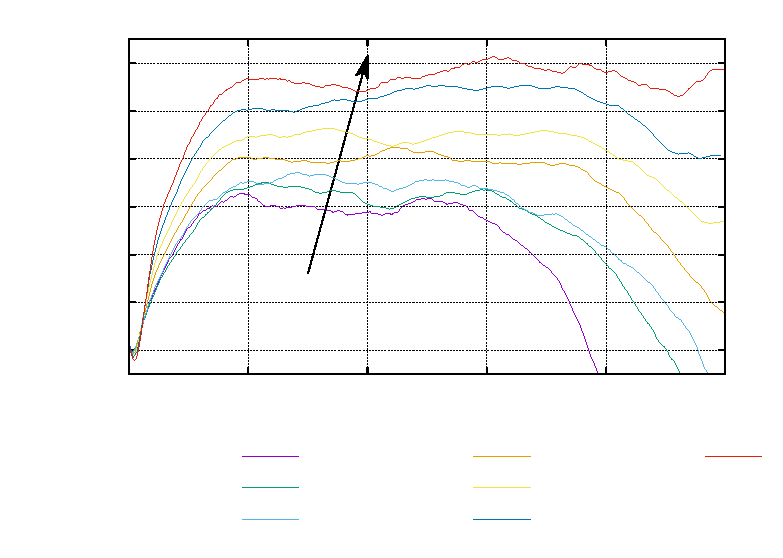
\includegraphics[width={360.00bp},height={252.00bp}]{./indiceVide}}%
    \gplfronttext
  \end{picture}%
\endgroup

                                    \caption{L'indice de vide}
                                \end{figure}
                                    
                                \begin{figure}
                                   % GNUPLOT: LaTeX picture with Postscript
\begingroup
  \makeatletter
  \providecommand\color[2][]{%
    \GenericError{(gnuplot) \space\space\space\@spaces}{%
      Package color not loaded in conjunction with
      terminal option `colourtext'%
    }{See the gnuplot documentation for explanation.%
    }{Either use 'blacktext' in gnuplot or load the package
      color.sty in LaTeX.}%
    \renewcommand\color[2][]{}%
  }%
  \providecommand\includegraphics[2][]{%
    \GenericError{(gnuplot) \space\space\space\@spaces}{%
      Package graphicx or graphics not loaded%
    }{See the gnuplot documentation for explanation.%
    }{The gnuplot epslatex terminal needs graphicx.sty or graphics.sty.}%
    \renewcommand\includegraphics[2][]{}%
  }%
  \providecommand\rotatebox[2]{#2}%
  \@ifundefined{ifGPcolor}{%
    \newif\ifGPcolor
    \GPcolortrue
  }{}%
  \@ifundefined{ifGPblacktext}{%
    \newif\ifGPblacktext
    \GPblacktextfalse
  }{}%
  % define a \g@addto@macro without @ in the name:
  \let\gplgaddtomacro\g@addto@macro
  % define empty templates for all commands taking text:
  \gdef\gplbacktext{}%
  \gdef\gplfronttext{}%
  \makeatother
  \ifGPblacktext
    % no textcolor at all
    \def\colorrgb#1{}%
    \def\colorgray#1{}%
  \else
    % gray or color?
    \ifGPcolor
      \def\colorrgb#1{\color[rgb]{#1}}%
      \def\colorgray#1{\color[gray]{#1}}%
      \expandafter\def\csname LTw\endcsname{\color{white}}%
      \expandafter\def\csname LTb\endcsname{\color{black}}%
      \expandafter\def\csname LTa\endcsname{\color{black}}%
      \expandafter\def\csname LT0\endcsname{\color[rgb]{1,0,0}}%
      \expandafter\def\csname LT1\endcsname{\color[rgb]{0,1,0}}%
      \expandafter\def\csname LT2\endcsname{\color[rgb]{0,0,1}}%
      \expandafter\def\csname LT3\endcsname{\color[rgb]{1,0,1}}%
      \expandafter\def\csname LT4\endcsname{\color[rgb]{0,1,1}}%
      \expandafter\def\csname LT5\endcsname{\color[rgb]{1,1,0}}%
      \expandafter\def\csname LT6\endcsname{\color[rgb]{0,0,0}}%
      \expandafter\def\csname LT7\endcsname{\color[rgb]{1,0.3,0}}%
      \expandafter\def\csname LT8\endcsname{\color[rgb]{0.5,0.5,0.5}}%
    \else
      % gray
      \def\colorrgb#1{\color{black}}%
      \def\colorgray#1{\color[gray]{#1}}%
      \expandafter\def\csname LTw\endcsname{\color{white}}%
      \expandafter\def\csname LTb\endcsname{\color{black}}%
      \expandafter\def\csname LTa\endcsname{\color{black}}%
      \expandafter\def\csname LT0\endcsname{\color{black}}%
      \expandafter\def\csname LT1\endcsname{\color{black}}%
      \expandafter\def\csname LT2\endcsname{\color{black}}%
      \expandafter\def\csname LT3\endcsname{\color{black}}%
      \expandafter\def\csname LT4\endcsname{\color{black}}%
      \expandafter\def\csname LT5\endcsname{\color{black}}%
      \expandafter\def\csname LT6\endcsname{\color{black}}%
      \expandafter\def\csname LT7\endcsname{\color{black}}%
      \expandafter\def\csname LT8\endcsname{\color{black}}%
    \fi
  \fi
    \setlength{\unitlength}{0.0500bp}%
    \ifx\gptboxheight\undefined%
      \newlength{\gptboxheight}%
      \newlength{\gptboxwidth}%
      \newsavebox{\gptboxtext}%
    \fi%
    \setlength{\fboxrule}{0.5pt}%
    \setlength{\fboxsep}{1pt}%
    \definecolor{tbcol}{rgb}{1,1,1}%
\begin{picture}(7200.00,5040.00)%
    \gplgaddtomacro\gplbacktext{%
      \csname LTb\endcsname%%
      \put(814,1604){\makebox(0,0)[r]{\strut{}$1$}}%
      \csname LTb\endcsname%%
      \put(814,1961){\makebox(0,0)[r]{\strut{}$1.5$}}%
      \csname LTb\endcsname%%
      \put(814,2318){\makebox(0,0)[r]{\strut{}$2$}}%
      \csname LTb\endcsname%%
      \put(814,2676){\makebox(0,0)[r]{\strut{}$2.5$}}%
      \csname LTb\endcsname%%
      \put(814,3033){\makebox(0,0)[r]{\strut{}$3$}}%
      \csname LTb\endcsname%%
      \put(814,3390){\makebox(0,0)[r]{\strut{}$3.5$}}%
      \csname LTb\endcsname%%
      \put(814,3747){\makebox(0,0)[r]{\strut{}$4$}}%
      \csname LTb\endcsname%%
      \put(814,4105){\makebox(0,0)[r]{\strut{}$4.5$}}%
      \csname LTb\endcsname%%
      \put(814,4462){\makebox(0,0)[r]{\strut{}$5$}}%
      \csname LTb\endcsname%%
      \put(814,4819){\makebox(0,0)[r]{\strut{}$5.5$}}%
      \csname LTb\endcsname%%
      \put(946,1384){\makebox(0,0){\strut{}$0$}}%
      \csname LTb\endcsname%%
      \put(2117,1384){\makebox(0,0){\strut{}$20$}}%
      \csname LTb\endcsname%%
      \put(3289,1384){\makebox(0,0){\strut{}$40$}}%
      \csname LTb\endcsname%%
      \put(4460,1384){\makebox(0,0){\strut{}$60$}}%
      \csname LTb\endcsname%%
      \put(5632,1384){\makebox(0,0){\strut{}$80$}}%
      \csname LTb\endcsname%%
      \put(6803,1384){\makebox(0,0){\strut{}$100$}}%
    }%
    \gplgaddtomacro\gplfronttext{%
      \csname LTb\endcsname%%
      \put(209,3211){\rotatebox{-270}{\makebox(0,0){\strut{}Z}}}%
      \put(3874,1054){\makebox(0,0){\strut{}$\varepsilon_{yy}$ (\%)}}%
      \csname LTb\endcsname%%
      \put(1980,813){\makebox(0,0)[r]{\strut{}$I = 1 \times 10^{-4}$}}%
      \csname LTb\endcsname%%
      \put(1980,513){\makebox(0,0)[r]{\strut{}$I = 1 \times 10^{-3}$}}%
      \csname LTb\endcsname%%
      \put(1980,213){\makebox(0,0)[r]{\strut{}$I = 2 \times 10^{-3}$}}%
      \csname LTb\endcsname%%
      \put(4203,813){\makebox(0,0)[r]{\strut{}$I = 4 \times 10^{-3}$}}%
      \csname LTb\endcsname%%
      \put(4203,513){\makebox(0,0)[r]{\strut{}$I = 6 \times 10^{-3}$}}%
      \csname LTb\endcsname%%
      \put(4203,213){\makebox(0,0)[r]{\strut{}$I = 8 \times 10^{-3}$}}%
      \csname LTb\endcsname%%
      \put(6426,813){\makebox(0,0)[r]{\strut{}$I = 1 \times 10^{-2}$}}%
    }%
    \gplbacktext
    \put(0,0){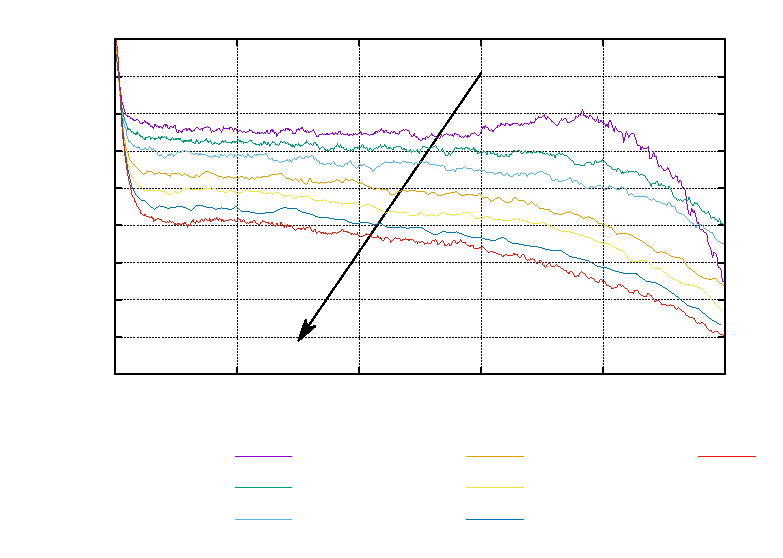
\includegraphics[width={360.00bp},height={252.00bp}]{./NombreCoordination}}%
    \gplfronttext
  \end{picture}%
\endgroup

                                    \caption{Nombre de coordination}
                                \end{figure}

                                Vitesse imposée est élevée $\rightarrow$ Contrainte de confinement et l'indice de vide sont instables

     
                                \begin{figure}
                                    % GNUPLOT: LaTeX picture with Postscript
\begingroup
  \makeatletter
  \providecommand\color[2][]{%
    \GenericError{(gnuplot) \space\space\space\@spaces}{%
      Package color not loaded in conjunction with
      terminal option `colourtext'%
    }{See the gnuplot documentation for explanation.%
    }{Either use 'blacktext' in gnuplot or load the package
      color.sty in LaTeX.}%
    \renewcommand\color[2][]{}%
  }%
  \providecommand\includegraphics[2][]{%
    \GenericError{(gnuplot) \space\space\space\@spaces}{%
      Package graphicx or graphics not loaded%
    }{See the gnuplot documentation for explanation.%
    }{The gnuplot epslatex terminal needs graphicx.sty or graphics.sty.}%
    \renewcommand\includegraphics[2][]{}%
  }%
  \providecommand\rotatebox[2]{#2}%
  \@ifundefined{ifGPcolor}{%
    \newif\ifGPcolor
    \GPcolortrue
  }{}%
  \@ifundefined{ifGPblacktext}{%
    \newif\ifGPblacktext
    \GPblacktextfalse
  }{}%
  % define a \g@addto@macro without @ in the name:
  \let\gplgaddtomacro\g@addto@macro
  % define empty templates for all commands taking text:
  \gdef\gplbacktext{}%
  \gdef\gplfronttext{}%
  \makeatother
  \ifGPblacktext
    % no textcolor at all
    \def\colorrgb#1{}%
    \def\colorgray#1{}%
  \else
    % gray or color?
    \ifGPcolor
      \def\colorrgb#1{\color[rgb]{#1}}%
      \def\colorgray#1{\color[gray]{#1}}%
      \expandafter\def\csname LTw\endcsname{\color{white}}%
      \expandafter\def\csname LTb\endcsname{\color{black}}%
      \expandafter\def\csname LTa\endcsname{\color{black}}%
      \expandafter\def\csname LT0\endcsname{\color[rgb]{1,0,0}}%
      \expandafter\def\csname LT1\endcsname{\color[rgb]{0,1,0}}%
      \expandafter\def\csname LT2\endcsname{\color[rgb]{0,0,1}}%
      \expandafter\def\csname LT3\endcsname{\color[rgb]{1,0,1}}%
      \expandafter\def\csname LT4\endcsname{\color[rgb]{0,1,1}}%
      \expandafter\def\csname LT5\endcsname{\color[rgb]{1,1,0}}%
      \expandafter\def\csname LT6\endcsname{\color[rgb]{0,0,0}}%
      \expandafter\def\csname LT7\endcsname{\color[rgb]{1,0.3,0}}%
      \expandafter\def\csname LT8\endcsname{\color[rgb]{0.5,0.5,0.5}}%
    \else
      % gray
      \def\colorrgb#1{\color{black}}%
      \def\colorgray#1{\color[gray]{#1}}%
      \expandafter\def\csname LTw\endcsname{\color{white}}%
      \expandafter\def\csname LTb\endcsname{\color{black}}%
      \expandafter\def\csname LTa\endcsname{\color{black}}%
      \expandafter\def\csname LT0\endcsname{\color{black}}%
      \expandafter\def\csname LT1\endcsname{\color{black}}%
      \expandafter\def\csname LT2\endcsname{\color{black}}%
      \expandafter\def\csname LT3\endcsname{\color{black}}%
      \expandafter\def\csname LT4\endcsname{\color{black}}%
      \expandafter\def\csname LT5\endcsname{\color{black}}%
      \expandafter\def\csname LT6\endcsname{\color{black}}%
      \expandafter\def\csname LT7\endcsname{\color{black}}%
      \expandafter\def\csname LT8\endcsname{\color{black}}%
    \fi
  \fi
    \setlength{\unitlength}{0.0500bp}%
    \ifx\gptboxheight\undefined%
      \newlength{\gptboxheight}%
      \newlength{\gptboxwidth}%
      \newsavebox{\gptboxtext}%
    \fi%
    \setlength{\fboxrule}{0.5pt}%
    \setlength{\fboxsep}{1pt}%
    \definecolor{tbcol}{rgb}{1,1,1}%
\begin{picture}(7200.00,5040.00)%
    \gplgaddtomacro\gplbacktext{%
      \csname LTb\endcsname%%
      \put(946,1584){\makebox(0,0)[r]{\strut{}$0$}}%
      \csname LTb\endcsname%%
      \put(946,2123){\makebox(0,0)[r]{\strut{}$200$}}%
      \csname LTb\endcsname%%
      \put(946,2662){\makebox(0,0)[r]{\strut{}$400$}}%
      \csname LTb\endcsname%%
      \put(946,3202){\makebox(0,0)[r]{\strut{}$600$}}%
      \csname LTb\endcsname%%
      \put(946,3741){\makebox(0,0)[r]{\strut{}$800$}}%
      \csname LTb\endcsname%%
      \put(946,4280){\makebox(0,0)[r]{\strut{}$1000$}}%
      \csname LTb\endcsname%%
      \put(946,4819){\makebox(0,0)[r]{\strut{}$1200$}}%
      \csname LTb\endcsname%%
      \put(1078,1364){\makebox(0,0){\strut{}$0$}}%
      \csname LTb\endcsname%%
      \put(1700,1364){\makebox(0,0){\strut{}$10$}}%
      \csname LTb\endcsname%%
      \put(2322,1364){\makebox(0,0){\strut{}$20$}}%
      \csname LTb\endcsname%%
      \put(2944,1364){\makebox(0,0){\strut{}$30$}}%
      \csname LTb\endcsname%%
      \put(3567,1364){\makebox(0,0){\strut{}$40$}}%
      \csname LTb\endcsname%%
      \put(4189,1364){\makebox(0,0){\strut{}$50$}}%
      \csname LTb\endcsname%%
      \put(4811,1364){\makebox(0,0){\strut{}$60$}}%
      \csname LTb\endcsname%%
      \put(5433,1364){\makebox(0,0){\strut{}$70$}}%
      \csname LTb\endcsname%%
      \put(6055,1364){\makebox(0,0){\strut{}$80$}}%
      \put(6187,1584){\makebox(0,0)[l]{\strut{}$-2$}}%
      \put(6187,1908){\makebox(0,0)[l]{\strut{}$-1$}}%
      \put(6187,2231){\makebox(0,0)[l]{\strut{}$0$}}%
      \put(6187,2555){\makebox(0,0)[l]{\strut{}$1$}}%
      \put(6187,2878){\makebox(0,0)[l]{\strut{}$2$}}%
      \put(6187,3202){\makebox(0,0)[l]{\strut{}$3$}}%
      \put(6187,3525){\makebox(0,0)[l]{\strut{}$4$}}%
      \put(6187,3849){\makebox(0,0)[l]{\strut{}$5$}}%
      \put(6187,4172){\makebox(0,0)[l]{\strut{}$6$}}%
      \put(6187,4496){\makebox(0,0)[l]{\strut{}$7$}}%
      \put(6187,4819){\makebox(0,0)[l]{\strut{}$8$}}%
    }%
    \gplgaddtomacro\gplfronttext{%
      \csname LTb\endcsname%%
      \put(341,3201){\rotatebox{-270}{\makebox(0,0){\strut{}q (kPa)}}}%
      \put(6693,3201){\rotatebox{-270}{\makebox(0,0){\strut{}$\varepsilon_v$ (\%)}}}%
      \put(3566,1034){\makebox(0,0){\strut{}$\varepsilon_{yy}$ (\%)}}%
      \csname LTb\endcsname%%
      \put(2711,833){\makebox(0,0)[r]{\strut{}$I = 1 \times 10^{-4}$}}%
      \csname LTb\endcsname%%
      \put(2711,613){\makebox(0,0)[r]{\strut{}$I = 1 \times 10^{-3}$}}%
      \csname LTb\endcsname%%
      \put(2711,393){\makebox(0,0)[r]{\strut{}$I = 2 \times 10^{-3}$}}%
      \csname LTb\endcsname%%
      \put(2711,173){\makebox(0,0)[r]{\strut{}$I = 4 \times 10^{-3}$}}%
      \csname LTb\endcsname%%
      \put(5150,833){\makebox(0,0)[r]{\strut{}$I = 6 \times 10^{-3}$}}%
      \csname LTb\endcsname%%
      \put(5150,613){\makebox(0,0)[r]{\strut{}$I = 8 \times 10^{-3}$}}%
      \csname LTb\endcsname%%
      \put(5150,393){\makebox(0,0)[r]{\strut{}$I = 1 \times 10^{-2}$}}%
    }%
    \gplbacktext
    \put(0,0){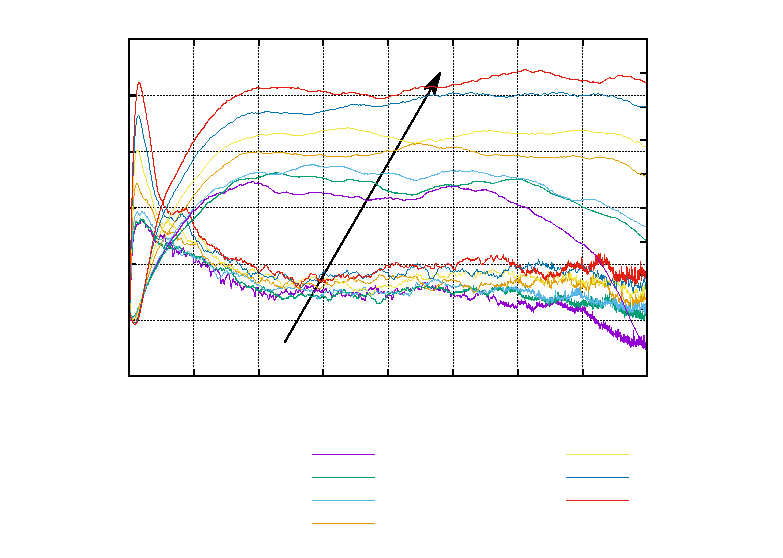
\includegraphics[width={360.00bp},height={252.00bp}]{./Test}}%
    \gplfronttext
  \end{picture}%
\endgroup

                                    \caption{Contrainte-Déformation}
                                \end{figure}
                                J'ai choisi $\varepsilon_{yy} = 70\%$ pour réaliser des pré-études sur la rhéologie $\mu(I)$ (considéré comme l'état critique). 


                                \begin{figure}
                                  % GNUPLOT: LaTeX picture with Postscript
\begingroup
  \makeatletter
  \providecommand\color[2][]{%
    \GenericError{(gnuplot) \space\space\space\@spaces}{%
      Package color not loaded in conjunction with
      terminal option `colourtext'%
    }{See the gnuplot documentation for explanation.%
    }{Either use 'blacktext' in gnuplot or load the package
      color.sty in LaTeX.}%
    \renewcommand\color[2][]{}%
  }%
  \providecommand\includegraphics[2][]{%
    \GenericError{(gnuplot) \space\space\space\@spaces}{%
      Package graphicx or graphics not loaded%
    }{See the gnuplot documentation for explanation.%
    }{The gnuplot epslatex terminal needs graphicx.sty or graphics.sty.}%
    \renewcommand\includegraphics[2][]{}%
  }%
  \providecommand\rotatebox[2]{#2}%
  \@ifundefined{ifGPcolor}{%
    \newif\ifGPcolor
    \GPcolortrue
  }{}%
  \@ifundefined{ifGPblacktext}{%
    \newif\ifGPblacktext
    \GPblacktextfalse
  }{}%
  % define a \g@addto@macro without @ in the name:
  \let\gplgaddtomacro\g@addto@macro
  % define empty templates for all commands taking text:
  \gdef\gplbacktext{}%
  \gdef\gplfronttext{}%
  \makeatother
  \ifGPblacktext
    % no textcolor at all
    \def\colorrgb#1{}%
    \def\colorgray#1{}%
  \else
    % gray or color?
    \ifGPcolor
      \def\colorrgb#1{\color[rgb]{#1}}%
      \def\colorgray#1{\color[gray]{#1}}%
      \expandafter\def\csname LTw\endcsname{\color{white}}%
      \expandafter\def\csname LTb\endcsname{\color{black}}%
      \expandafter\def\csname LTa\endcsname{\color{black}}%
      \expandafter\def\csname LT0\endcsname{\color[rgb]{1,0,0}}%
      \expandafter\def\csname LT1\endcsname{\color[rgb]{0,1,0}}%
      \expandafter\def\csname LT2\endcsname{\color[rgb]{0,0,1}}%
      \expandafter\def\csname LT3\endcsname{\color[rgb]{1,0,1}}%
      \expandafter\def\csname LT4\endcsname{\color[rgb]{0,1,1}}%
      \expandafter\def\csname LT5\endcsname{\color[rgb]{1,1,0}}%
      \expandafter\def\csname LT6\endcsname{\color[rgb]{0,0,0}}%
      \expandafter\def\csname LT7\endcsname{\color[rgb]{1,0.3,0}}%
      \expandafter\def\csname LT8\endcsname{\color[rgb]{0.5,0.5,0.5}}%
    \else
      % gray
      \def\colorrgb#1{\color{black}}%
      \def\colorgray#1{\color[gray]{#1}}%
      \expandafter\def\csname LTw\endcsname{\color{white}}%
      \expandafter\def\csname LTb\endcsname{\color{black}}%
      \expandafter\def\csname LTa\endcsname{\color{black}}%
      \expandafter\def\csname LT0\endcsname{\color{black}}%
      \expandafter\def\csname LT1\endcsname{\color{black}}%
      \expandafter\def\csname LT2\endcsname{\color{black}}%
      \expandafter\def\csname LT3\endcsname{\color{black}}%
      \expandafter\def\csname LT4\endcsname{\color{black}}%
      \expandafter\def\csname LT5\endcsname{\color{black}}%
      \expandafter\def\csname LT6\endcsname{\color{black}}%
      \expandafter\def\csname LT7\endcsname{\color{black}}%
      \expandafter\def\csname LT8\endcsname{\color{black}}%
    \fi
  \fi
    \setlength{\unitlength}{0.0500bp}%
    \ifx\gptboxheight\undefined%
      \newlength{\gptboxheight}%
      \newlength{\gptboxwidth}%
      \newsavebox{\gptboxtext}%
    \fi%
    \setlength{\fboxrule}{0.5pt}%
    \setlength{\fboxsep}{1pt}%
    \definecolor{tbcol}{rgb}{1,1,1}%
\begin{picture}(7200.00,5040.00)%
    \gplgaddtomacro\gplbacktext{%
      \csname LTb\endcsname%%
      \put(814,1881){\makebox(0,0)[r]{\strut{}$0$}}%
      \put(814,2299){\makebox(0,0)[r]{\strut{}$100$}}%
      \put(814,2718){\makebox(0,0)[r]{\strut{}$200$}}%
      \put(814,3136){\makebox(0,0)[r]{\strut{}$300$}}%
      \put(814,3554){\makebox(0,0)[r]{\strut{}$400$}}%
      \put(814,3973){\makebox(0,0)[r]{\strut{}$500$}}%
      \put(946,1661){\makebox(0,0){\strut{}$0$}}%
      \put(1783,1661){\makebox(0,0){\strut{}$200$}}%
      \put(2619,1661){\makebox(0,0){\strut{}$400$}}%
      \put(3456,1661){\makebox(0,0){\strut{}$600$}}%
      \put(4293,1661){\makebox(0,0){\strut{}$800$}}%
      \put(5130,1661){\makebox(0,0){\strut{}$1000$}}%
      \put(5966,1661){\makebox(0,0){\strut{}$1200$}}%
      \put(6803,1661){\makebox(0,0){\strut{}$1400$}}%
    }%
    \gplgaddtomacro\gplfronttext{%
      \csname LTb\endcsname%%
      \put(209,3031){\rotatebox{-270}{\makebox(0,0){\strut{}$\tau$ (kPa)}}}%
      \put(3874,1331){\makebox(0,0){\strut{}$\sigma_n$ (kPa)}}%
      \csname LTb\endcsname%%
      \put(2160,513){\makebox(0,0)[r]{\strut{}$I = 1 \times 10^{-4}$}}%
      \csname LTb\endcsname%%
      \put(2160,333){\makebox(0,0)[r]{\strut{}$I = 1 \times 10^{-3}$}}%
      \csname LTb\endcsname%%
      \put(2160,153){\makebox(0,0)[r]{\strut{}$I = 2 \times 10^{-3}$}}%
      \csname LTb\endcsname%%
      \put(4167,513){\makebox(0,0)[r]{\strut{}$I = 4 \times 10^{-3}$}}%
      \csname LTb\endcsname%%
      \put(4167,333){\makebox(0,0)[r]{\strut{}$I = 6 \times 10^{-3}$}}%
      \csname LTb\endcsname%%
      \put(4167,153){\makebox(0,0)[r]{\strut{}$I = 8 \times 10^{-3}$}}%
      \csname LTb\endcsname%%
      \put(6174,513){\makebox(0,0)[r]{\strut{}$I = 1 \times 10^{-2}$}}%
    }%
    \gplbacktext
    \put(0,0){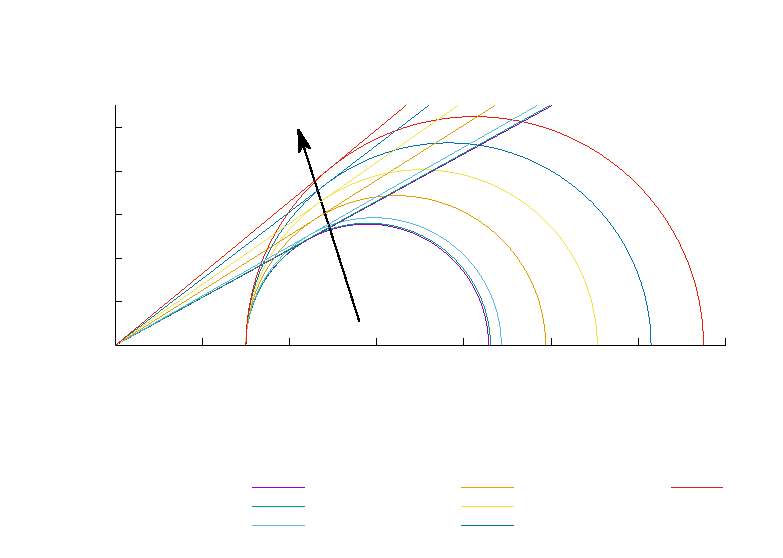
\includegraphics[width={360.00bp},height={252.00bp}]{Transitoire}}%
    \gplfronttext
  \end{picture}%
\endgroup

                                    \caption{Cercle transitore (pic)}
                                \end{figure}

                                    $\varphi = 28.77^\circ \div 39.53^\circ $


                                \begin{figure}
                                    \input{Résiduel.tex}
                                    \caption{Cercle résiduel ($\varepsilon_{yy} = 70\%$)}
                                \end{figure}
                                    $\varphi = 16.56^\circ \div 22.78^\circ $
                                    
\section{Comparaison des équations utilisées}

Expérimental : 
\[
I =  \dfrac{\dot{\varepsilon} \cdot \bar{a}}{\sqrt{\sigma_{33}/\rho_s}}; \quad \mu = \sin(\varphi)
\]

Simulation : 
\[
I = \dot{\varepsilon} \times \sqrt {\dfrac{m}{\sigma_{33}\times \bar{a}}}  
= \dot{\varepsilon} \times \sqrt {\dfrac{\dfrac{4}{3} \pi \dfrac{\bar{a}^3}{8} \times \rho_s}{\sigma_{33}\times \bar{a}}} 
= \dot{\varepsilon} \times \sqrt{\dfrac{\pi}{6}} \sqrt {\dfrac{\bar{a}^2 \rho_s}{\sigma_{33}}} 
= \boxed{\sqrt{\dfrac{\pi}{6}}} \times \dfrac{\dot{\varepsilon} \cdot \bar{a}}{\sqrt{\sigma_{33}/\rho_s}}
\]
\[
\mu = \tan(\varphi)
\]

\section{Rhéologie $\mu(I)$ résiduel}

\subsection{Première méthode}

La première méthode utilise les équations suivantes :
\[
\mu(I) = \mu_s + \dfrac{\mu_2 - \mu_s}{1 + \dfrac{I_0}{I}}
\]
\[
\Phi(I) = \Phi^{\max} - bI
\]

Les coefficients $\mu_s,\ \mu_2,\ I_0,\ \Phi_{\max},\ b$ sont déterminés empiriquement.

\begin{figure}
    \centering
    {\small
        % GNUPLOT: LaTeX picture with Postscript
\begingroup
  \makeatletter
  \providecommand\color[2][]{%
    \GenericError{(gnuplot) \space\space\space\@spaces}{%
      Package color not loaded in conjunction with
      terminal option `colourtext'%
    }{See the gnuplot documentation for explanation.%
    }{Either use 'blacktext' in gnuplot or load the package
      color.sty in LaTeX.}%
    \renewcommand\color[2][]{}%
  }%
  \providecommand\includegraphics[2][]{%
    \GenericError{(gnuplot) \space\space\space\@spaces}{%
      Package graphicx or graphics not loaded%
    }{See the gnuplot documentation for explanation.%
    }{The gnuplot epslatex terminal needs graphicx.sty or graphics.sty.}%
    \renewcommand\includegraphics[2][]{}%
  }%
  \providecommand\rotatebox[2]{#2}%
  \@ifundefined{ifGPcolor}{%
    \newif\ifGPcolor
    \GPcolortrue
  }{}%
  \@ifundefined{ifGPblacktext}{%
    \newif\ifGPblacktext
    \GPblacktextfalse
  }{}%
  % define a \g@addto@macro without @ in the name:
  \let\gplgaddtomacro\g@addto@macro
  % define empty templates for all commands taking text:
  \gdef\gplbacktext{}%
  \gdef\gplfronttext{}%
  \makeatother
  \ifGPblacktext
    % no textcolor at all
    \def\colorrgb#1{}%
    \def\colorgray#1{}%
  \else
    % gray or color?
    \ifGPcolor
      \def\colorrgb#1{\color[rgb]{#1}}%
      \def\colorgray#1{\color[gray]{#1}}%
      \expandafter\def\csname LTw\endcsname{\color{white}}%
      \expandafter\def\csname LTb\endcsname{\color{black}}%
      \expandafter\def\csname LTa\endcsname{\color{black}}%
      \expandafter\def\csname LT0\endcsname{\color[rgb]{1,0,0}}%
      \expandafter\def\csname LT1\endcsname{\color[rgb]{0,1,0}}%
      \expandafter\def\csname LT2\endcsname{\color[rgb]{0,0,1}}%
      \expandafter\def\csname LT3\endcsname{\color[rgb]{1,0,1}}%
      \expandafter\def\csname LT4\endcsname{\color[rgb]{0,1,1}}%
      \expandafter\def\csname LT5\endcsname{\color[rgb]{1,1,0}}%
      \expandafter\def\csname LT6\endcsname{\color[rgb]{0,0,0}}%
      \expandafter\def\csname LT7\endcsname{\color[rgb]{1,0.3,0}}%
      \expandafter\def\csname LT8\endcsname{\color[rgb]{0.5,0.5,0.5}}%
    \else
      % gray
      \def\colorrgb#1{\color{black}}%
      \def\colorgray#1{\color[gray]{#1}}%
      \expandafter\def\csname LTw\endcsname{\color{white}}%
      \expandafter\def\csname LTb\endcsname{\color{black}}%
      \expandafter\def\csname LTa\endcsname{\color{black}}%
      \expandafter\def\csname LT0\endcsname{\color{black}}%
      \expandafter\def\csname LT1\endcsname{\color{black}}%
      \expandafter\def\csname LT2\endcsname{\color{black}}%
      \expandafter\def\csname LT3\endcsname{\color{black}}%
      \expandafter\def\csname LT4\endcsname{\color{black}}%
      \expandafter\def\csname LT5\endcsname{\color{black}}%
      \expandafter\def\csname LT6\endcsname{\color{black}}%
      \expandafter\def\csname LT7\endcsname{\color{black}}%
      \expandafter\def\csname LT8\endcsname{\color{black}}%
    \fi
  \fi
    \setlength{\unitlength}{0.0500bp}%
    \ifx\gptboxheight\undefined%
      \newlength{\gptboxheight}%
      \newlength{\gptboxwidth}%
      \newsavebox{\gptboxtext}%
    \fi%
    \setlength{\fboxrule}{0.5pt}%
    \setlength{\fboxsep}{1pt}%
    \definecolor{tbcol}{rgb}{1,1,1}%
\begin{picture}(7200.00,5040.00)%
    \gplgaddtomacro\gplbacktext{%
      \csname LTb\endcsname%%
      \put(946,704){\makebox(0,0)[r]{\strut{}$0.28$}}%
      \csname LTb\endcsname%%
      \put(946,1161){\makebox(0,0)[r]{\strut{}$0.3$}}%
      \csname LTb\endcsname%%
      \put(946,1618){\makebox(0,0)[r]{\strut{}$0.32$}}%
      \csname LTb\endcsname%%
      \put(946,2076){\makebox(0,0)[r]{\strut{}$0.34$}}%
      \csname LTb\endcsname%%
      \put(946,2533){\makebox(0,0)[r]{\strut{}$0.36$}}%
      \csname LTb\endcsname%%
      \put(946,2990){\makebox(0,0)[r]{\strut{}$0.38$}}%
      \csname LTb\endcsname%%
      \put(946,3447){\makebox(0,0)[r]{\strut{}$0.4$}}%
      \csname LTb\endcsname%%
      \put(946,3905){\makebox(0,0)[r]{\strut{}$0.42$}}%
      \csname LTb\endcsname%%
      \put(946,4362){\makebox(0,0)[r]{\strut{}$0.44$}}%
      \csname LTb\endcsname%%
      \put(946,4819){\makebox(0,0)[r]{\strut{}$0.46$}}%
      \csname LTb\endcsname%%
      \put(1078,484){\makebox(0,0){\strut{}$10^{-4}$}}%
      \csname LTb\endcsname%%
      \put(2986,484){\makebox(0,0){\strut{}$10^{-3}$}}%
      \csname LTb\endcsname%%
      \put(4895,484){\makebox(0,0){\strut{}$10^{-2}$}}%
      \csname LTb\endcsname%%
      \put(6803,484){\makebox(0,0){\strut{}$10^{-1}$}}%
      \put(1651,3996){\makebox(0,0)[l]{\strut{}$\mu_s = 0.2953$}}%
      \put(1651,3585){\makebox(0,0)[l]{\strut{}$\mu_2 = 0.5329$}}%
      \put(1651,3173){\makebox(0,0)[l]{\strut{}$I_0 = 0.0483$}}%
    }%
    \gplgaddtomacro\gplfronttext{%
      \csname LTb\endcsname%%
      \put(209,2761){\rotatebox{-270}{\makebox(0,0){\strut{}$\mu$}}}%
      \put(3940,154){\makebox(0,0){\strut{}$I$}}%
      \csname LTb\endcsname%%
      \put(3322,4646){\makebox(0,0)[r]{\strut{}Données}}%
      \csname LTb\endcsname%%
      \put(3322,4426){\makebox(0,0)[r]{\strut{}$\mu(I)$ régression}}%
    }%
    \gplbacktext
    \put(0,0){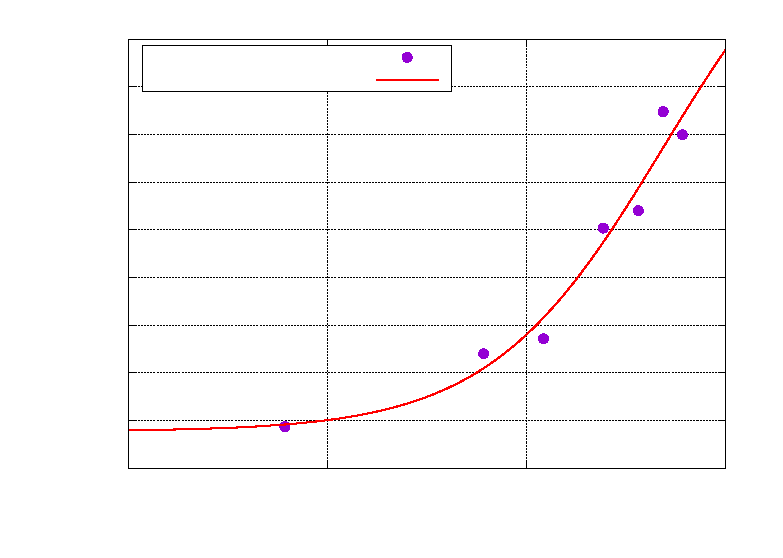
\includegraphics[width={360.00bp},height={252.00bp}]{./mu_I_fit}}%
    \gplfronttext
  \end{picture}%
\endgroup

    }
    \caption{$\mu(I)$ ($\varepsilon_{yy} = 70\%$)}
\end{figure}

\begin{figure}
    \centering
    {\small
        % GNUPLOT: LaTeX picture with Postscript
\begingroup
  \makeatletter
  \providecommand\color[2][]{%
    \GenericError{(gnuplot) \space\space\space\@spaces}{%
      Package color not loaded in conjunction with
      terminal option `colourtext'%
    }{See the gnuplot documentation for explanation.%
    }{Either use 'blacktext' in gnuplot or load the package
      color.sty in LaTeX.}%
    \renewcommand\color[2][]{}%
  }%
  \providecommand\includegraphics[2][]{%
    \GenericError{(gnuplot) \space\space\space\@spaces}{%
      Package graphicx or graphics not loaded%
    }{See the gnuplot documentation for explanation.%
    }{The gnuplot epslatex terminal needs graphicx.sty or graphics.sty.}%
    \renewcommand\includegraphics[2][]{}%
  }%
  \providecommand\rotatebox[2]{#2}%
  \@ifundefined{ifGPcolor}{%
    \newif\ifGPcolor
    \GPcolortrue
  }{}%
  \@ifundefined{ifGPblacktext}{%
    \newif\ifGPblacktext
    \GPblacktextfalse
  }{}%
  % define a \g@addto@macro without @ in the name:
  \let\gplgaddtomacro\g@addto@macro
  % define empty templates for all commands taking text:
  \gdef\gplbacktext{}%
  \gdef\gplfronttext{}%
  \makeatother
  \ifGPblacktext
    % no textcolor at all
    \def\colorrgb#1{}%
    \def\colorgray#1{}%
  \else
    % gray or color?
    \ifGPcolor
      \def\colorrgb#1{\color[rgb]{#1}}%
      \def\colorgray#1{\color[gray]{#1}}%
      \expandafter\def\csname LTw\endcsname{\color{white}}%
      \expandafter\def\csname LTb\endcsname{\color{black}}%
      \expandafter\def\csname LTa\endcsname{\color{black}}%
      \expandafter\def\csname LT0\endcsname{\color[rgb]{1,0,0}}%
      \expandafter\def\csname LT1\endcsname{\color[rgb]{0,1,0}}%
      \expandafter\def\csname LT2\endcsname{\color[rgb]{0,0,1}}%
      \expandafter\def\csname LT3\endcsname{\color[rgb]{1,0,1}}%
      \expandafter\def\csname LT4\endcsname{\color[rgb]{0,1,1}}%
      \expandafter\def\csname LT5\endcsname{\color[rgb]{1,1,0}}%
      \expandafter\def\csname LT6\endcsname{\color[rgb]{0,0,0}}%
      \expandafter\def\csname LT7\endcsname{\color[rgb]{1,0.3,0}}%
      \expandafter\def\csname LT8\endcsname{\color[rgb]{0.5,0.5,0.5}}%
    \else
      % gray
      \def\colorrgb#1{\color{black}}%
      \def\colorgray#1{\color[gray]{#1}}%
      \expandafter\def\csname LTw\endcsname{\color{white}}%
      \expandafter\def\csname LTb\endcsname{\color{black}}%
      \expandafter\def\csname LTa\endcsname{\color{black}}%
      \expandafter\def\csname LT0\endcsname{\color{black}}%
      \expandafter\def\csname LT1\endcsname{\color{black}}%
      \expandafter\def\csname LT2\endcsname{\color{black}}%
      \expandafter\def\csname LT3\endcsname{\color{black}}%
      \expandafter\def\csname LT4\endcsname{\color{black}}%
      \expandafter\def\csname LT5\endcsname{\color{black}}%
      \expandafter\def\csname LT6\endcsname{\color{black}}%
      \expandafter\def\csname LT7\endcsname{\color{black}}%
      \expandafter\def\csname LT8\endcsname{\color{black}}%
    \fi
  \fi
    \setlength{\unitlength}{0.0500bp}%
    \ifx\gptboxheight\undefined%
      \newlength{\gptboxheight}%
      \newlength{\gptboxwidth}%
      \newsavebox{\gptboxtext}%
    \fi%
    \setlength{\fboxrule}{0.5pt}%
    \setlength{\fboxsep}{1pt}%
    \definecolor{tbcol}{rgb}{1,1,1}%
\begin{picture}(7200.00,5040.00)%
    \gplgaddtomacro\gplbacktext{%
      \csname LTb\endcsname%%
      \put(1078,704){\makebox(0,0)[r]{\strut{}$0.555$}}%
      \csname LTb\endcsname%%
      \put(1078,1116){\makebox(0,0)[r]{\strut{}$0.56$}}%
      \csname LTb\endcsname%%
      \put(1078,1527){\makebox(0,0)[r]{\strut{}$0.565$}}%
      \csname LTb\endcsname%%
      \put(1078,1939){\makebox(0,0)[r]{\strut{}$0.57$}}%
      \csname LTb\endcsname%%
      \put(1078,2350){\makebox(0,0)[r]{\strut{}$0.575$}}%
      \csname LTb\endcsname%%
      \put(1078,2762){\makebox(0,0)[r]{\strut{}$0.58$}}%
      \csname LTb\endcsname%%
      \put(1078,3173){\makebox(0,0)[r]{\strut{}$0.585$}}%
      \csname LTb\endcsname%%
      \put(1078,3585){\makebox(0,0)[r]{\strut{}$0.59$}}%
      \csname LTb\endcsname%%
      \put(1078,3996){\makebox(0,0)[r]{\strut{}$0.595$}}%
      \csname LTb\endcsname%%
      \put(1078,4408){\makebox(0,0)[r]{\strut{}$0.6$}}%
      \csname LTb\endcsname%%
      \put(1078,4819){\makebox(0,0)[r]{\strut{}$0.605$}}%
      \csname LTb\endcsname%%
      \put(1210,484){\makebox(0,0){\strut{}$10^{-4}$}}%
      \csname LTb\endcsname%%
      \put(3074,484){\makebox(0,0){\strut{}$10^{-3}$}}%
      \csname LTb\endcsname%%
      \put(4939,484){\makebox(0,0){\strut{}$10^{-2}$}}%
      \csname LTb\endcsname%%
      \put(6803,484){\makebox(0,0){\strut{}$10^{-1}$}}%
      \put(1769,1733){\makebox(0,0)[l]{\strut{}$\Phi_{max} = 0.6019$}}%
      \put(1769,1321){\makebox(0,0)[l]{\strut{}$b = 0.4641$}}%
    }%
    \gplgaddtomacro\gplfronttext{%
      \csname LTb\endcsname%%
      \put(209,2761){\rotatebox{-270}{\makebox(0,0){\strut{}$\Phi$}}}%
      \put(4006,154){\makebox(0,0){\strut{}$I$}}%
      \csname LTb\endcsname%%
      \put(3454,1097){\makebox(0,0)[r]{\strut{}Données}}%
      \csname LTb\endcsname%%
      \put(3454,877){\makebox(0,0)[r]{\strut{}$\Phi(I)$ régression}}%
    }%
    \gplbacktext
    \put(0,0){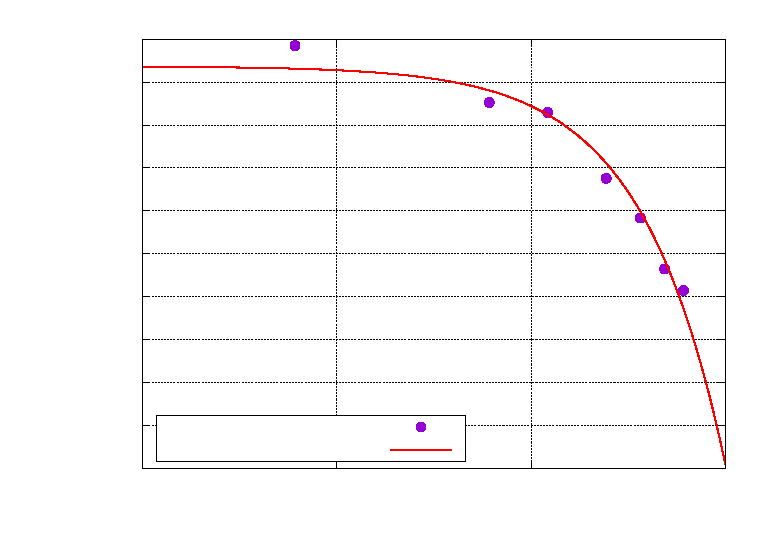
\includegraphics[width={360.00bp},height={252.00bp}]{./Pack_I_fit}}%
    \gplfronttext
  \end{picture}%
\endgroup

    }
    \caption{$\Phi(I)$ ($\varepsilon_{yy} = 70\%$)}
\end{figure}

\subsection{Deuxième méthode}

La deuxième méthode, proposée dans l'article 
\href{https://link-springer-com.sid2nomade-1.grenet.fr/article/10.1007/s10035-024-01459-7}{Scaling laws for quasi-statically deforming granular soil at critical state [2024] (Fei, Jianbo et al.)}, 
introduit un nombre d'inertie quasi-statique $Q$ qui tient compte du degré de compaction $\Phi_0$ :

\[
Q = \left[ \Phi_0  \ln \left( I \right) + \alpha \right]
\]
où $\alpha = 30$.

\[
\mu = \xi Q + C
\]

Les coefficients $\xi,\ C,\ \Phi_0$ sont déterminés empiriquement ($\xi \approx 0.06$ et $C \approx 0.2$).

\begin{figure}
    \centering
    {\small
        % GNUPLOT: LaTeX picture with Postscript
\begingroup
  \makeatletter
  \providecommand\color[2][]{%
    \GenericError{(gnuplot) \space\space\space\@spaces}{%
      Package color not loaded in conjunction with
      terminal option `colourtext'%
    }{See the gnuplot documentation for explanation.%
    }{Either use 'blacktext' in gnuplot or load the package
      color.sty in LaTeX.}%
    \renewcommand\color[2][]{}%
  }%
  \providecommand\includegraphics[2][]{%
    \GenericError{(gnuplot) \space\space\space\@spaces}{%
      Package graphicx or graphics not loaded%
    }{See the gnuplot documentation for explanation.%
    }{The gnuplot epslatex terminal needs graphicx.sty or graphics.sty.}%
    \renewcommand\includegraphics[2][]{}%
  }%
  \providecommand\rotatebox[2]{#2}%
  \@ifundefined{ifGPcolor}{%
    \newif\ifGPcolor
    \GPcolortrue
  }{}%
  \@ifundefined{ifGPblacktext}{%
    \newif\ifGPblacktext
    \GPblacktextfalse
  }{}%
  % define a \g@addto@macro without @ in the name:
  \let\gplgaddtomacro\g@addto@macro
  % define empty templates for all commands taking text:
  \gdef\gplbacktext{}%
  \gdef\gplfronttext{}%
  \makeatother
  \ifGPblacktext
    % no textcolor at all
    \def\colorrgb#1{}%
    \def\colorgray#1{}%
  \else
    % gray or color?
    \ifGPcolor
      \def\colorrgb#1{\color[rgb]{#1}}%
      \def\colorgray#1{\color[gray]{#1}}%
      \expandafter\def\csname LTw\endcsname{\color{white}}%
      \expandafter\def\csname LTb\endcsname{\color{black}}%
      \expandafter\def\csname LTa\endcsname{\color{black}}%
      \expandafter\def\csname LT0\endcsname{\color[rgb]{1,0,0}}%
      \expandafter\def\csname LT1\endcsname{\color[rgb]{0,1,0}}%
      \expandafter\def\csname LT2\endcsname{\color[rgb]{0,0,1}}%
      \expandafter\def\csname LT3\endcsname{\color[rgb]{1,0,1}}%
      \expandafter\def\csname LT4\endcsname{\color[rgb]{0,1,1}}%
      \expandafter\def\csname LT5\endcsname{\color[rgb]{1,1,0}}%
      \expandafter\def\csname LT6\endcsname{\color[rgb]{0,0,0}}%
      \expandafter\def\csname LT7\endcsname{\color[rgb]{1,0.3,0}}%
      \expandafter\def\csname LT8\endcsname{\color[rgb]{0.5,0.5,0.5}}%
    \else
      % gray
      \def\colorrgb#1{\color{black}}%
      \def\colorgray#1{\color[gray]{#1}}%
      \expandafter\def\csname LTw\endcsname{\color{white}}%
      \expandafter\def\csname LTb\endcsname{\color{black}}%
      \expandafter\def\csname LTa\endcsname{\color{black}}%
      \expandafter\def\csname LT0\endcsname{\color{black}}%
      \expandafter\def\csname LT1\endcsname{\color{black}}%
      \expandafter\def\csname LT2\endcsname{\color{black}}%
      \expandafter\def\csname LT3\endcsname{\color{black}}%
      \expandafter\def\csname LT4\endcsname{\color{black}}%
      \expandafter\def\csname LT5\endcsname{\color{black}}%
      \expandafter\def\csname LT6\endcsname{\color{black}}%
      \expandafter\def\csname LT7\endcsname{\color{black}}%
      \expandafter\def\csname LT8\endcsname{\color{black}}%
    \fi
  \fi
    \setlength{\unitlength}{0.0500bp}%
    \ifx\gptboxheight\undefined%
      \newlength{\gptboxheight}%
      \newlength{\gptboxwidth}%
      \newsavebox{\gptboxtext}%
    \fi%
    \setlength{\fboxrule}{0.5pt}%
    \setlength{\fboxsep}{1pt}%
    \definecolor{tbcol}{rgb}{1,1,1}%
\begin{picture}(7200.00,5040.00)%
    \gplgaddtomacro\gplbacktext{%
      \csname LTb\endcsname%%
      \put(946,704){\makebox(0,0)[r]{\strut{}$0.24$}}%
      \csname LTb\endcsname%%
      \put(946,1218){\makebox(0,0)[r]{\strut{}$0.26$}}%
      \csname LTb\endcsname%%
      \put(946,1733){\makebox(0,0)[r]{\strut{}$0.28$}}%
      \csname LTb\endcsname%%
      \put(946,2247){\makebox(0,0)[r]{\strut{}$0.3$}}%
      \csname LTb\endcsname%%
      \put(946,2762){\makebox(0,0)[r]{\strut{}$0.32$}}%
      \csname LTb\endcsname%%
      \put(946,3276){\makebox(0,0)[r]{\strut{}$0.34$}}%
      \csname LTb\endcsname%%
      \put(946,3790){\makebox(0,0)[r]{\strut{}$0.36$}}%
      \csname LTb\endcsname%%
      \put(946,4305){\makebox(0,0)[r]{\strut{}$0.38$}}%
      \csname LTb\endcsname%%
      \put(946,4819){\makebox(0,0)[r]{\strut{}$0.4$}}%
      \csname LTb\endcsname%%
      \put(1078,484){\makebox(0,0){\strut{}$10.5$}}%
      \csname LTb\endcsname%%
      \put(2032,484){\makebox(0,0){\strut{}$11$}}%
      \csname LTb\endcsname%%
      \put(2986,484){\makebox(0,0){\strut{}$11.5$}}%
      \csname LTb\endcsname%%
      \put(3941,484){\makebox(0,0){\strut{}$12$}}%
      \csname LTb\endcsname%%
      \put(4895,484){\makebox(0,0){\strut{}$12.5$}}%
      \csname LTb\endcsname%%
      \put(5849,484){\makebox(0,0){\strut{}$13$}}%
      \csname LTb\endcsname%%
      \put(6803,484){\makebox(0,0){\strut{}$13.5$}}%
      \put(1651,3996){\makebox(0,0)[l]{\strut{}$\xi = 0.0485$}}%
      \put(1651,3585){\makebox(0,0)[l]{\strut{}$c = -0.2636$}}%
      \put(1651,3173){\makebox(0,0)[l]{\strut{}$\Phi_0 = 0.4868$}}%
    }%
    \gplgaddtomacro\gplfronttext{%
      \csname LTb\endcsname%%
      \put(209,2761){\rotatebox{-270}{\makebox(0,0){\strut{}$\mu$}}}%
      \put(3940,154){\makebox(0,0){\strut{}$Q$}}%
      \csname LTb\endcsname%%
      \put(3322,4646){\makebox(0,0)[r]{\strut{}Données}}%
      \csname LTb\endcsname%%
      \put(3322,4426){\makebox(0,0)[r]{\strut{}$\mu(Q)$ régression}}%
    }%
    \gplbacktext
    \put(0,0){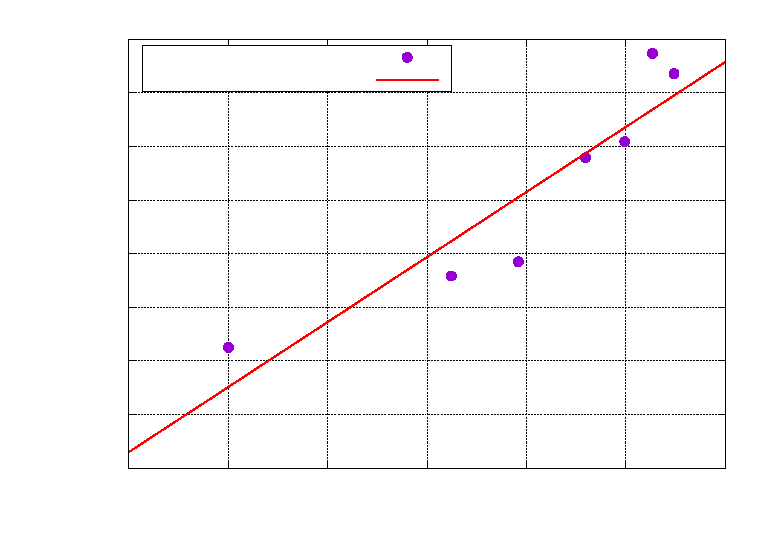
\includegraphics[width={360.00bp},height={252.00bp}]{./Q_mu}}%
    \gplfronttext
  \end{picture}%
\endgroup

    }
    \caption{$\mu(Q)$ avec $Q = f(\Phi_0, I)$}
\end{figure}


\bibliographystyle{plain}
\bibliography{Bibliographie}


\end{document}


